\documentclass[10pt,twocolumn,letterpaper]{article}

\usepackage{float}
\usepackage[caption = false]{subfig}
\usepackage[final]{graphicx}


\usepackage{cvpr}
\usepackage{times}
\usepackage{epsfig}
\usepackage{graphicx}
\usepackage{amsmath}
\usepackage{amssymb}

% Include other packages here, before hyperref.

% If you comment hyperref and then uncomment it, you should delete
% egpaper.aux before re-running latex.  (Or just hit 'q' on the first latex
% run, let it finish, and you should be clear).
\usepackage[breaklinks=true,bookmarks=false]{hyperref}

\cvprfinalcopy % *** Uncomment this line for the final submission

\def\cvprPaperID{****} % *** Enter the CVPR Paper ID here
\def\httilde{\mbox{\tt\raisebox{-.5ex}{\symbol{126}}}}

\begin{document}

%%%%%%%%% TITLE
\title{CUTIE: Learning to Understand Documents with Convolutional Universal Text Information Extractor}

\author{
  Xiaohui Zhao, Zhuo Wu, and Xiaoguang Wang \\
  New IT Accenture \\
{\tt\small xiaohui.zhao@accenture.com zhuo.wu@accenture.com danny.x.wang@accenture.com}
% Additional authors and addresses can be added with ``\and'',
}

\maketitle
%\thispagestyle{empty}

%%%%%%%%% ABSTRACT
\begin{abstract}
   Extracting key information from documents, such as receipts or invoices, and preserving the interested texts to structured data is crucial in the document-intensive streamline processes of office automation in areas that includes but not limited to accounting, financial, and taxation areas. Large proportion of published works attempt to tackle the problem by exploring the semantic context in text sequences based on the Named Entity Recognition (NER) method in the NLP field. In this paper, we propose to combine the effective information from both semantic meaning and spatial distribution of texts in documents. Specifically, our proposed model, Convolutional Universal Text Information Extractor (CUTIE), applies convolutional neural networks on the gridded texts where texts are embedded as features with semantical connotations. We further explore the effect of employing different structures of convolutional neural network and propose a fast and portable structure. We demonstrate the effectiveness of the proposed method on a dataset with up to $6,980$ labelled receipts, without any pre-training or post-processing, achieving state of the art performance that is much higher than BERT but with only $1/9$ parameters and without requiring the $3,300$M word dataset for pre-training.
\end{abstract}

%%%%%%%%% BODY TEXT
\section{Introduction}

Implementing Scanned receipts OCR and information extraction (SROIE) is of great benefit to services and applications such as efficient archiving, compliance check, and fast indexing in the document-intensive streamline processes of office automation in areas that includes but not limit to accounting, financial, and taxation areas. There are two specific tasks involved in SROIE: receipt OCR and key information extraction. In this work, we focus on the second task that is rare in published research. In fact, key information extraction faces big challenges, where different types of document structures and vast number of potential interested key words introduces great difficulties. Although the commonly used rule-based method can be implemented with carefully designed expert rules, it can only work on specific type of documents and takes no lesser effort to adapt to new type of documents. Therefore, it is desirable to have a learning-based key information extraction method with limited requirement of human resources and solely employing the deep learning technique without designing expert rules for any specific type of documents. 

History about published learning-based methods goes here.
The majority of the published learning-based works are based on the Named Entity Recognition (NER) research in the NLP field that is not originally designed to solve the key information extraction problem in SROIE, which align text words in the original document as a long paragraph in line-based rule. However, the real-world documents, such as receipts and invoices, present with various styles of layouts that were designed for different scenarios or from different enterprise entities. The order or word-to-word distance of the texts in the line-based aligned long paragraph tend to vary greatly due to layout variations, which is difficult to be handled with the natural language paragraph oriented methods, one typical example is illustrated in Fig. \ref{fig:receipts}.

\begin{figure*}
\begin{center}
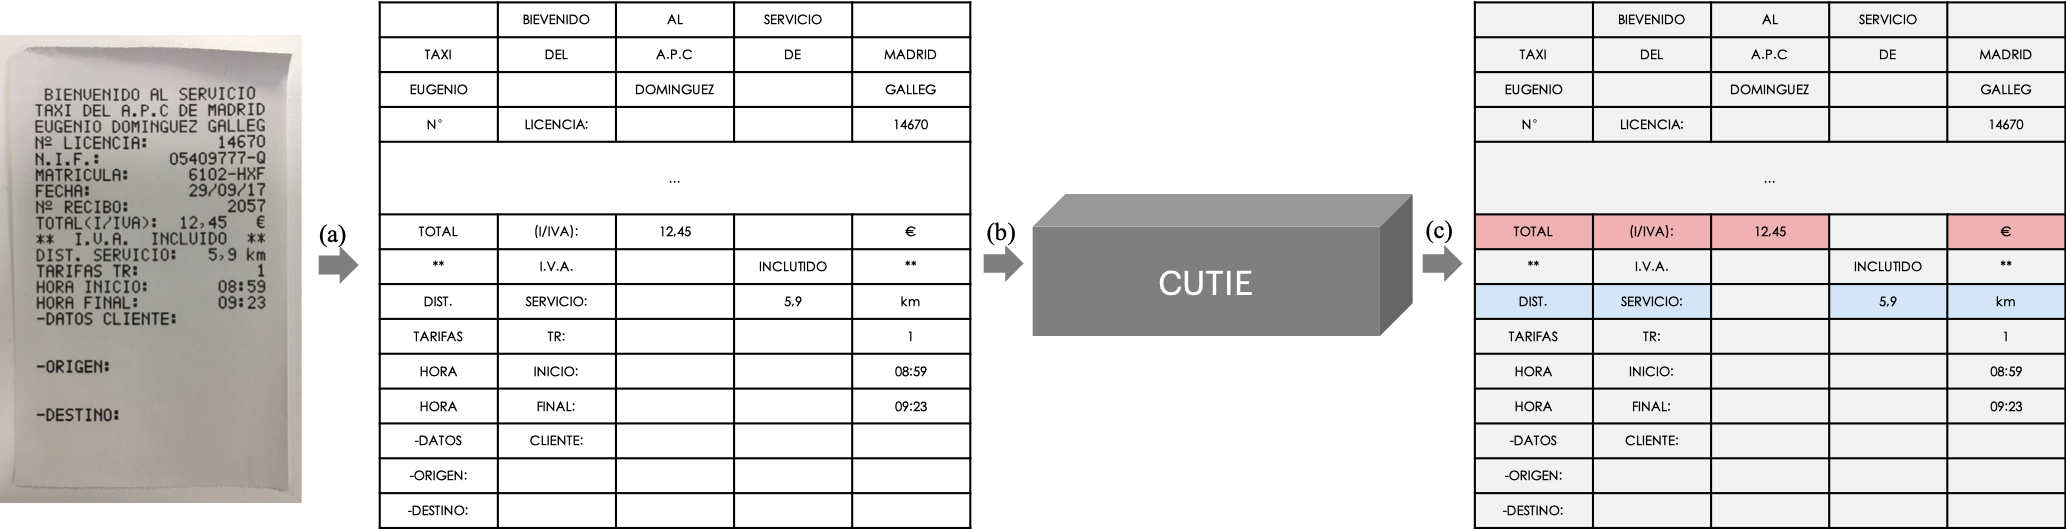
\includegraphics[width=0.99\linewidth]{Model.png}
\end{center}
   \caption{Framework of the proposed method, (a) positional map the scanned document image to a grid with text's relative spatial relation preserved, (b) feed the generated grid into the CNN for extracting key information, (c) reverse map the extracted key information for visual reference.}
\label{fig:cutie}
\end{figure*}
In this work, attempting to involve the spatial information into the key information extraction process, we propose to tackle this problem by using the CNN based network structure and involve the semantic features in a properly designed fashion. In particular, our proposed model, called Convolutional Universal Text Information Extractor (CUTIE), tackles the key information extraction problem by applying convolutional deep learning model on the gridded texts, as illustrated in Fig. \ref{fig:cutie}. The gridded texts is formed with the proposed grid positional mapping method, where the grid is generated with the principle that is preserving text's relative spatial relationship in the original scanned document image. The rich semantic information is encoded from the gridded texts at the very beginning stage of the convolutional neural network with a word embedding layer. The CUTIE allows for simultaneously looking into both semantical information and spatial information of the texts in the scanned document image and can reach a new state of the art result for key information extraction, which outperforms BERT model but without demand pretraining on a huge text dataset \cite{bert,transformer}.


\section{Related Work}


\section{Methods}
In this section, we introduce the method proposed for creating grid data for model training. We then present the network architectures that capture long distance information and avoid information loss in the convolutional neural networks that have striding or pooling processes.

\subsection{Grid Positional Mapping}
\label{pm}
To generate input grid data for the convolutional neural network, the scanned document image are processed by an OCR engine to acquire the texts and their absolute / relative positions. Let the scanned document image be of shape $(w, h)$, the minimum bounding box around the $i$-th interested text $s_i$ be $b_i$ that is restricted by two corner coordinates, where the upper-left corner coordinate in the scanned document be $(x^i_{left}, y^i_{top})$ and the bottom right of the bounding box be $(x^i_{right}, y^i_{bottom})$. To avoid the affects from overlapped bounding boxes and reveal the actual relative position among texts, we calculate the center point $(c^i_x, c^i_y)$ of the bounding boxes as the reference position. It is not hard to find that involving pre-processes that combine texts into meaningful entities will benefit the grid positional mapping process. However, this is not the major purpose of this paper and we leave it to future researches. In this paper, we tokenize the text words with a greedy longest-match-first algorithm using a pre-defined dictionary \cite{bertgit}. 

Let the grid positional mapping process be $G$ and the target grid size be $(c_{g_m}, r_{g_m})$. To generate the grid data, the goal of $G$ is to map the texts from the original scanned document image to the target grid, such that the mapped grid preserves the original spatial relationship among texts yet more suitable to be used as the input for the convolutional neural network. The mapping position of texts in the grid is calculated as

\begin{equation}
\label{cx}
c^i_x = c_{g_m} \frac{x_{left} + \frac{(x_{right} - x_{left})}{2}}{w}
\end{equation}
\begin{equation}
\label{cy}
r^i_y = r_{g_m} \frac{y_{top} + \frac{(y_{bottom} - y_{top})}{2}}{h}
\end{equation}

For tokenized texts, the bounding box is horizontally divided into multiple boxes and their row and col reference positions are calculated using the same criteria as Equ. \ref{cx} and Equ. \ref{cy}, separately. Furthermore, to enhance the capability of CUTIE to better handle documents with different layouts, we augment the grid data to shapes with different rows and columns by random sampling a Gaussian distribution for with probability

\begin{equation}
\label{augmentc}
p_c(k) = \frac{1}{\sqrt{2 \pi \sigma^2}} e^{- \frac{(k - c_{g_t})^2}{2 \sigma^2}}
\end{equation}
\begin{equation}
\label{augmentr}
p_r(k) = \frac{1}{\sqrt{2 \pi \sigma^2}} e^{- \frac{(k - r_{g_t})^2}{2 \sigma^2}}
\end{equation}
where $c_{g_t}$ is the mean center of the target augment gird size, $r_{g_t}$ is the mean center of the target augment grid size, and $\sigma$ is the standard deviation.


\subsection{CUTIE Model}
Through matching the output of CUTIE with the labelled grid data, the model learns to generate the label for each text in the grid input via exploring both the spatial and semantic features. For that reason, the task of CUTIE bears resemblance to the semantic segmentation task in the computer vision field but with more sparse data distributions. Specifically, the mapped grid contains scattered data points (text tokens) in contrast to the images bespread with pixels. The grid positional mapped key texts are either close to or distant to each other due to different types of document layouts. Therefore, incorporating multi-scale context processing ability benefits the network.

In fact, several methods have been proposed in the semantic segmentation field to capture multi-scale contexts in the input data. The methods of image pyramid and the encoder-decoder structure both aim at exploiting multi-scale information. The interested objects from different scales become prominent in the former networks by using multiple scaled input data to gather multi-scale features. The later networks shrink feature maps to enlarge receptive fields and reduce computation burdens, and then capture finer details by gradually recovering the spatial information from lower layer features. However, spatial resolution is reduced in the encoding process and the decoding process exploits only high resolution but low-level features to recover the spatial resolution, the consecutive striding encoding process decimates detail information \cite{hrnet}. Moreover, the encoding and decoding process applies shape restricts to the grid shape augment process as introduced in Section \ref{pm}. 

Instead, the field of view of filters can also be effectively enlarged and multi-scale contexts can be captured by combining multi-resolution features \cite{hrnet} or by applying atrous convolution \cite{deeplab, deeplabv1, deeplabv3, deeplabv3p}. To capture long distance connection and avoid potential information loss in the encoding process, we propose two different network architectures and compare their performance in Section \ref{experiment}. We had experimented with various types of model structures and only detail two of them here to avoid being a tedious paper. Specifically, proposed CUTIE-A is a high capacity convolutional neural network that fuses multi-resolution features without losing high-resolution features, proposed CUTIE-B is a convolutional network with atrous convolution for enlarging field of view and Atrous Spatial Pyramid Pooling (ASPP) module to capture multi-scale contexts. 

Both CUTIE-A and CUITE-B conducts semantical meaning encoding process with a word embedding layer in the very beginning stage. The cross entropy loss function is applied to compare the predicted token class grid and the ground truth grid.

\subsubsection{CUTIE-A}
CUTIE-A avoids information loss in the encoding process while taking advantage of encoders by combining encoding results to the maintained high-resolution representations through the entire convolutional process. Similar to HRNet proposed in \cite{hrnet}, a high-resolution network without striding is employed as the backbone network and several high-to-low resolution sub networks are gradually added and connected to the backbone major network. During the connecting process of the major network and sub networks, multi-scale features are fused to generate rich representations.

\subsubsection{CUTIE-B}
CUTIE-B is constructed with a single backbone network but employs atrous convolution to capture long distance connections. For atrous convolution, let the input feature map be $m$, filter be $w$ and output be $n$, for each position $i$, atrous convolution is applied over the input feature map $m$ as 

\begin{equation}
n[i] = \sum_k m[i+r\cdot k]w[k]
\end{equation}
where $r$ is the atrous rate that indicates the sampling stride of the input signal, which is implemented as convolving the input feature with up sampled filters by inserting $r-1$ zeros between two consecutive filter values along each spatial dimension. Standard convolution is a special case of atrous convolution with $r=1$ \cite{deeplabv1}.

\section{Experiments}
\label{experiment}
The proposed method is evaluated on a dataset with $3$ types of scanned document images, which contain $8$ key information classes and $1$ don't care class. For each specific key information class, multiple tokens can be included. The overall performance is referred as strict average precision (AP) and measured in terms of per-class accuracy across the $9$ classes, where one class is determined as correct only when every single token in the class is correct. To achieve deeper analysis of the performance of the proposed method, we propose to use one more criteria, soft average precision (softAP), where the prediction of a key information class is determined as correct as if positive ground truths are correctly predicted even if some false positive are included in the final prediction. SoftAP is important since it indicates model's capability of extracting correct key information with tolerance of incorporating certain false positives. In fact, post processing can be employed to eliminate the false positives. Therefore, joint analysis of AP and softAP provides a better understanding of the model performance.

\begin{figure}
\begin{center}
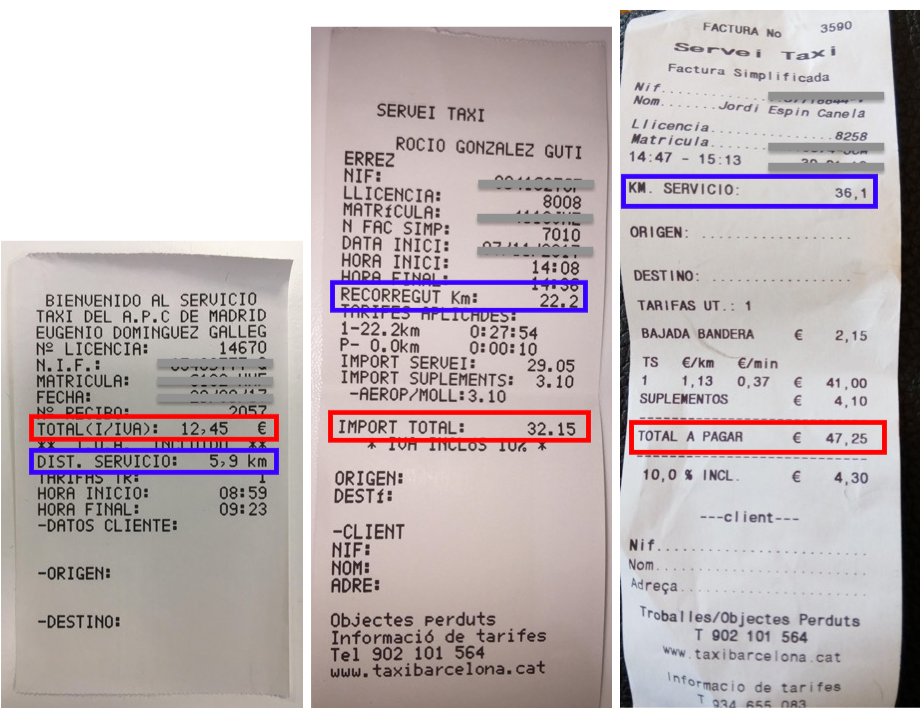
\includegraphics[width=0.99\linewidth]{Receipts.png}
\end{center}
   \caption{Example of scanned taxi receipt images. We provide two colored rectangles to help readers find the key information about distance of travel and total amount with blue and red, respectively. Note the different types of spatial layouts and key information texts in these receipt images.}
\label{fig:receipts}
\end{figure}

We compare the performance of the proposed method with two state of the art methods CloudScan \cite{cloudscan} and BERT \cite{bert}. For comparison, the Cloud Scan model for SROIE is trained from scratch but with several expert designed features as described in \cite{cloudscan}. The BERT model for SROIE is transform learned with the Google released base model that is pre-trained on a huge dataset with $3,300$M words \cite{bert,bertgit}.

We use a learning rate of $1e-3$ with Adam optimizer and step decay learning strategy. The learning rate is dropped to $1e-4$ and $1e-5$ on the $15,000$-th and $30,000$-th steps, respectively. The training is terminated within $40,000$ steps with batch size of $32$. Instance normalization is involved to facilate training. Our model is trained end-to-end without piecewise pretraining of any component. The embedding size is $128$, target augmentation shape is $64$ for both row and column. The dataset is split as training set and test set with ratio of $75:25$.

\subsection{Dataset}
The dataset contains $6,980$ annotated scanned Spanish receipt documents, including taxi receipts, meals entertainment (ME) receipts, and hotel receipts, with $9$ different key information classes, as reported in Table \ref{tab:dataset}. We generate the texts and corresponding bounding boxes with Google's OCR API. Each text and their bounding box is manually labelled as one of the $9$ different classes: 'DontCare', 'VendorName', 'VendorTaxID', 'InvoiceDate', 'InvoiceNumber', 'ExpenseAmount', 'BaseAmount', 'TaxAmount', and 'TaxRate'. We then employ the tokenizer introduced in Section \ref{pm} to segment texts into minimum token units, where text bounding boxes are also segmented accordingly. 

The dataset in this work is much more difficult than the neat scanned document images, since various layouts of receipts were captured in different scenarios using ordinary mobile phone camera. Examples of the scanned document images in our dataset are illustrated in Figure \ref{fig:receipts}, note that the colored rectangles is only for visual reference and the actual labelled data is in token-level rather than the line-level that is shown in the figure.
\begin{table}
	\caption{Statistic of the numbers of labelled receipt document images and key information classes in the dataset.}
\begin{center}
\begin{tabular}{l | c | c | c}
	 & Training Set & Test Set & \#classes \\
	\hline
	ME & 1109 & 475 & 9 \\
	Taxi & 2514 & 1077 & 6 \\
	Hotel & 1353 & 452 & 9 \\
\end{tabular}
\end{center}
	\label{tab:dataset}
\end{table}
\begin{table*}
	\caption{Performance comparison on different types of documents. (AP / softAP)}
\begin{center}
\begin{tabular}{l | c | c | c | c}
	Method & \#Params & Taxi & ME & Hotel \\
	\hline
	CloudScan\cite{cloudscan} & - & 82 / - & 64 / - & 60 / - \\
	BERT\cite{bert} & 110M & 87.0 / - & 80.3 / - & \textbf{79.4} / - \\
	CUTIE-A & 67M & / & \textbf{84.8} / \textbf{93.5} & / \\
	CUTIE-B & \textbf{14M} & \textbf{92.8} / \textbf{98.0} & 84.3 / 91.5 & 70.8 / \textbf{83.8} \\
\end{tabular}
\end{center}
	\label{tab:comparison}
\end{table*}

\subsection{Results on Validation Set}
We report results of our method in terms of AP and compare with other state of the art methods in Table \ref{tab:comparison}. We also provides softAP results for CUTIE-A and CUTIE-B in Table \ref{tab:comparison}, where both the softAP of CUTIE-A and CUTIE-B exceeds their AP by a large margin.  Examples of inference results are illustrated in Figure \ref{fig:result}. Our big network CUTIE-A achieves $100\%$ AP and $100\%$ softAP on meals entertainment receipts, $100\%$ AP and $100\%$ softAP on taxi receipts, and $100\%$ AP and $100\%$ softAP on hotel receipts, outperforming other methods in almost all of the test cases. Compared to CloudScan, our big network CUTIE-A improves AP by $100\%$ on meals entertainment receipts, $100\%$ on taxi receipt, and $100\%$ on hotel receipts; our small network CUTIE-B improves AP by $100\%$ points on meals entertainment receipts, $100$ on taxi receipts, and $100\%$ on hotel receipts. Furthermore, compared to BERT, where model is pre-trained on a dataset with $3,300M$ words and transfer learned on our dataset, our big network CUTIE-B improves AP by $100\%~100\%$ in meals entertainment and taxi receipts while using only $1/2$ parameters, our small network CUTIE-B improves AP by $100\%~100\%$ in meals entertainment and taxi receipts but with much less complexity and smaller model size with only $1/9$ parameters without requiring a huge dataset for model pretraining. 

It is worth noting that the difference of AP in the hotel receipt column actually leads to interesting findings. One of the finding is that if we neglect the 'VendorName' class in the evaluation criteria, the AP is increased to from $70.8\%$ to $76.9\%$ and the softAP drops to $83.8\%$, indicating that CUTIE is capable of extracting the interested 'VendorName' texts but sometimes involves texts that are not in the ground truth label. Another finding is that the hotel receipts are quite different from the meals entertainment receipts and the taxi receipts, where key information appear multi times in different areas of the receipt, whereas the human labelers tend to label only one of their appearances. We look deeper into this in the following part of this section by analyzing some error cases.
\begin{figure*}
\begin{center}
\subfloat{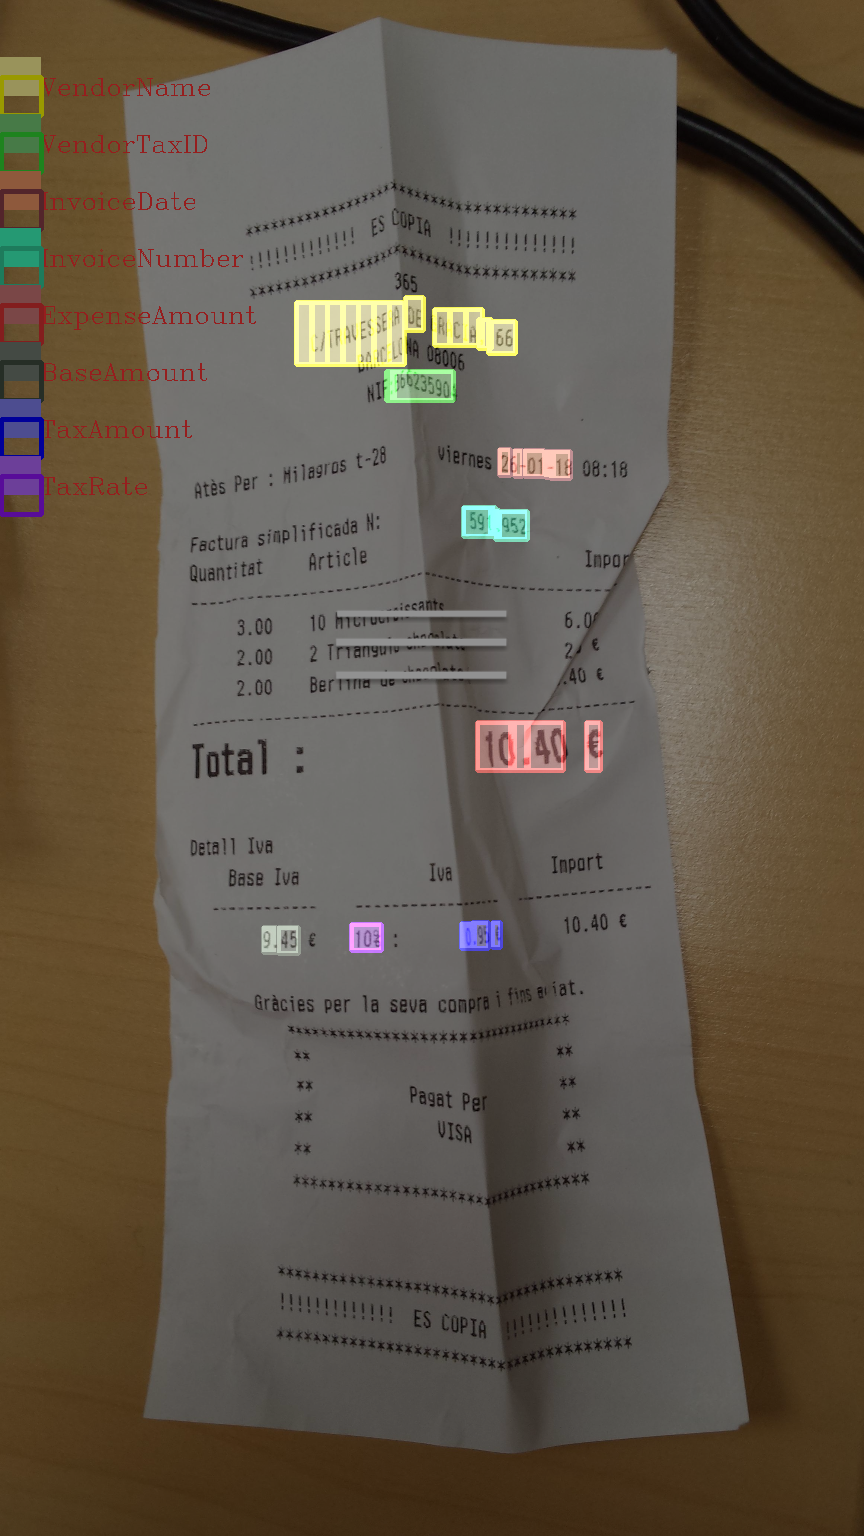
\includegraphics[width=0.17\linewidth]{appendix/meals/Correct_0.png}} 
\subfloat{\fcolorbox{white}{white}{}}
\subfloat{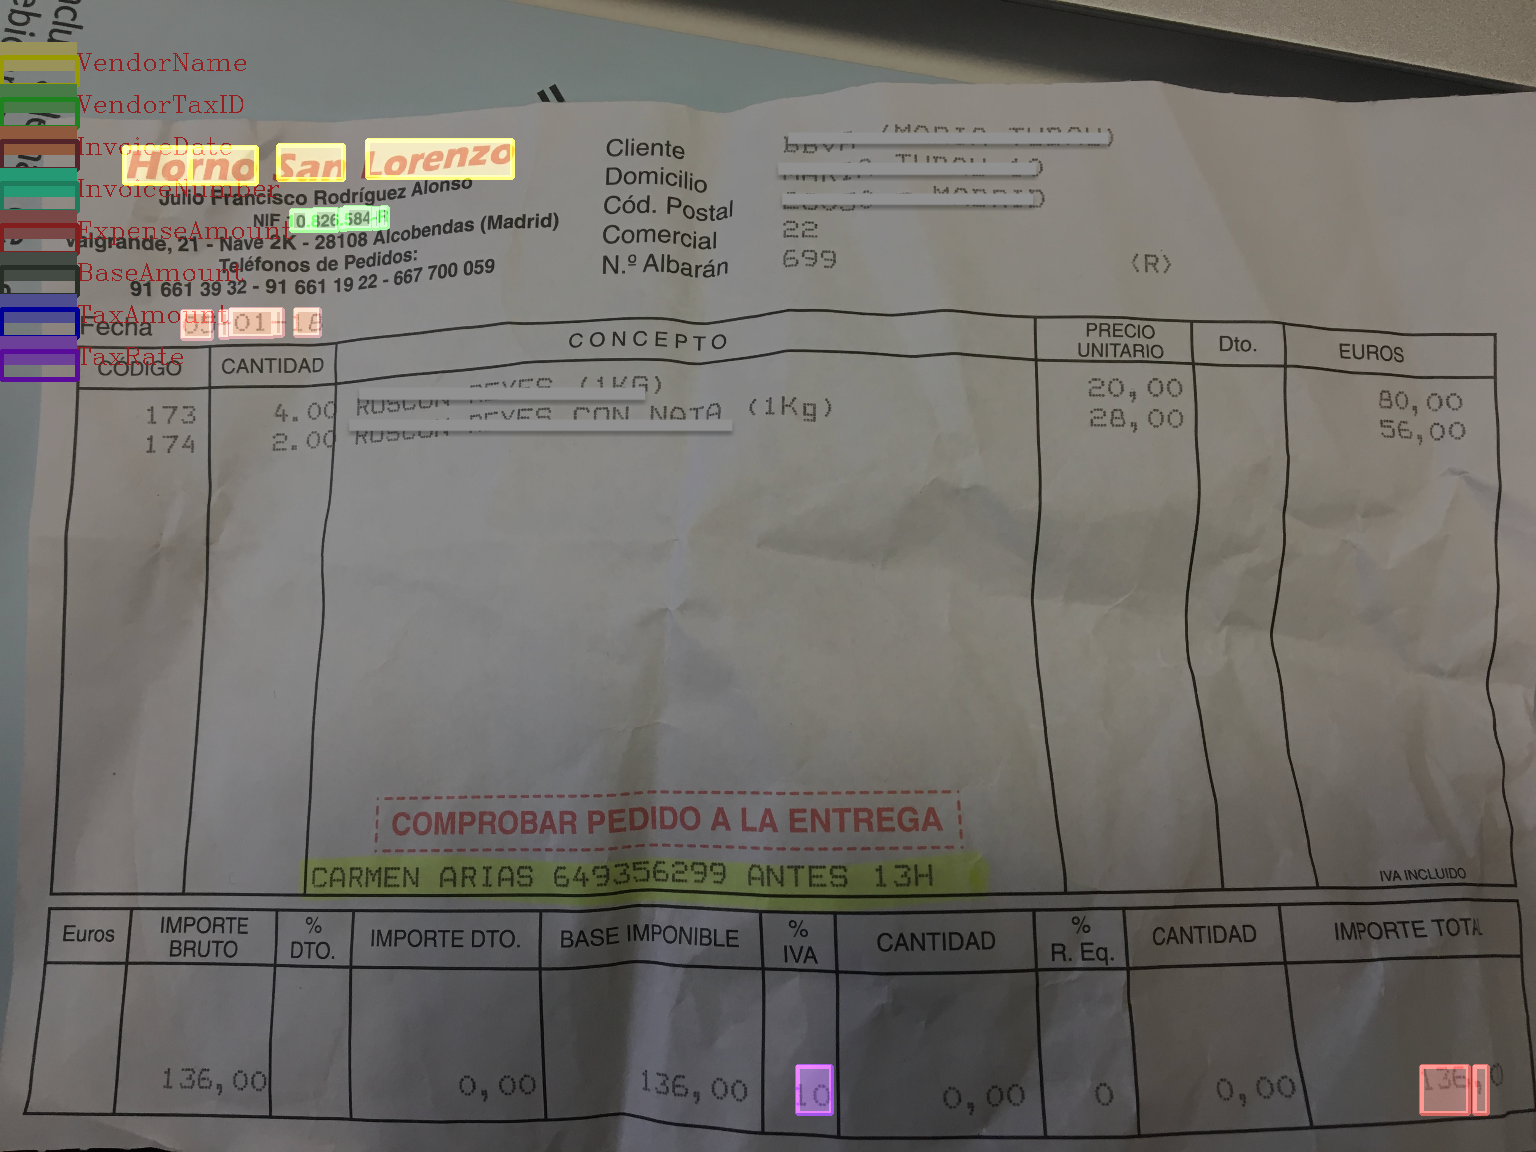
\includegraphics[width=0.39\linewidth]{appendix/meals/Correct_1.png}}
\subfloat{\fcolorbox{white}{white}{}}
\subfloat{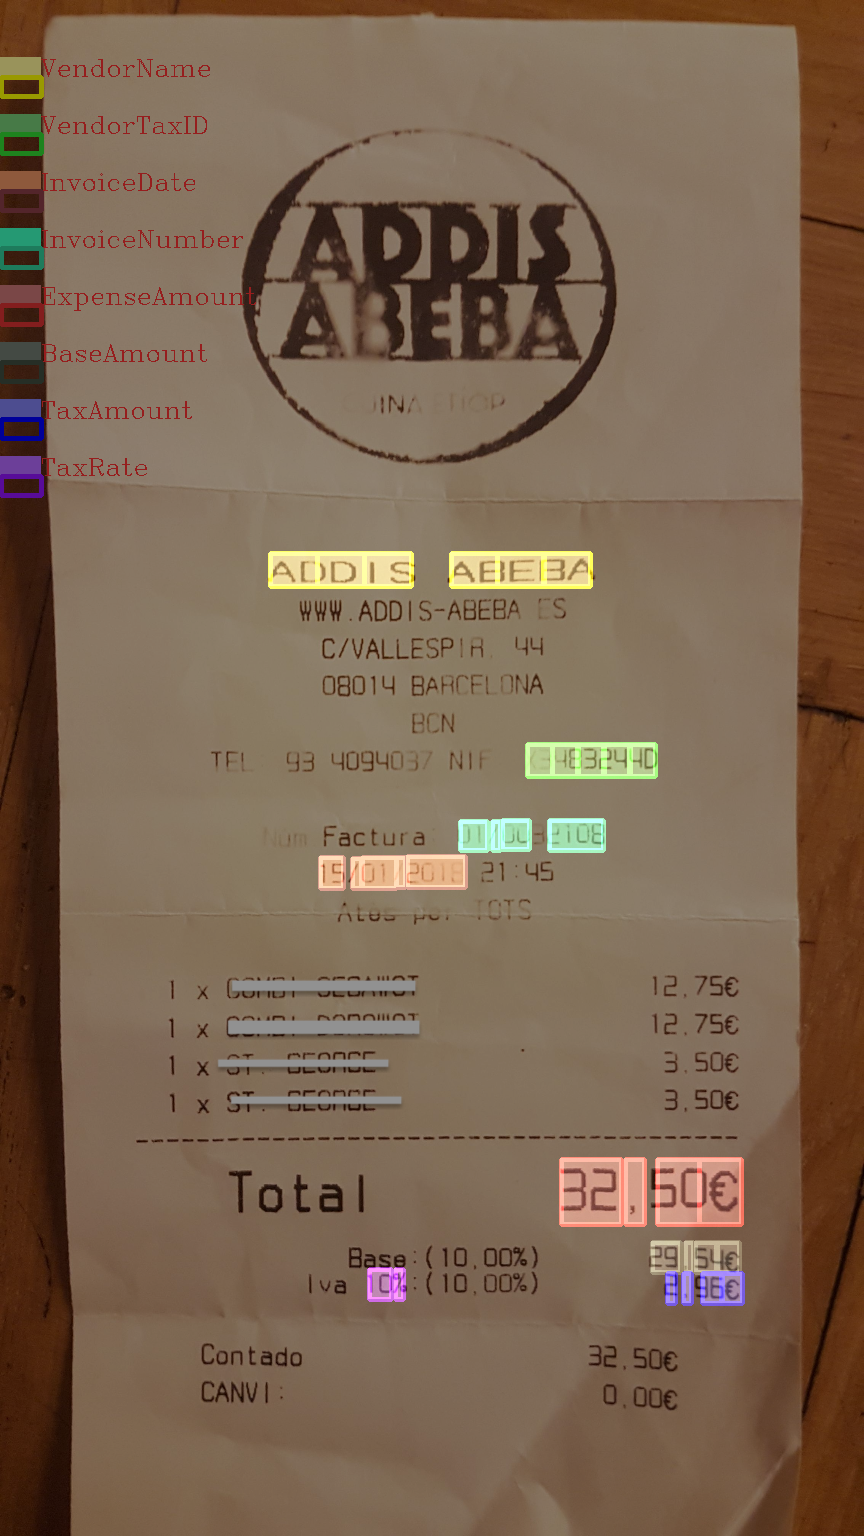
\includegraphics[width=0.17\linewidth]{appendix/meals/Correct_2.png}}
\subfloat{\fcolorbox{white}{white}{}}
\subfloat{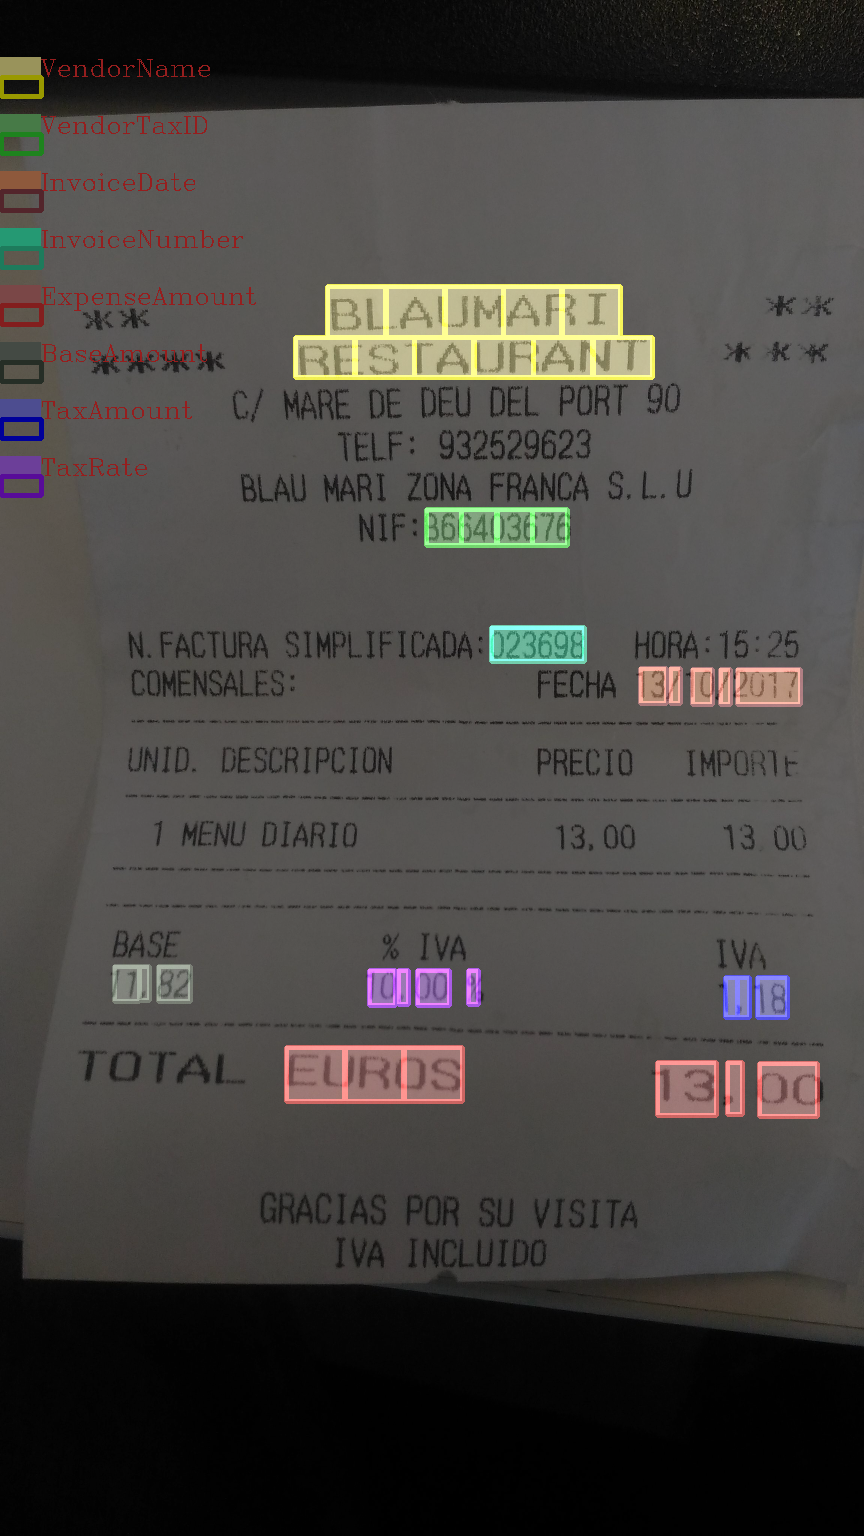
\includegraphics[width=0.17\linewidth]{appendix/meals/Correct_3.png}} \\ 
\subfloat{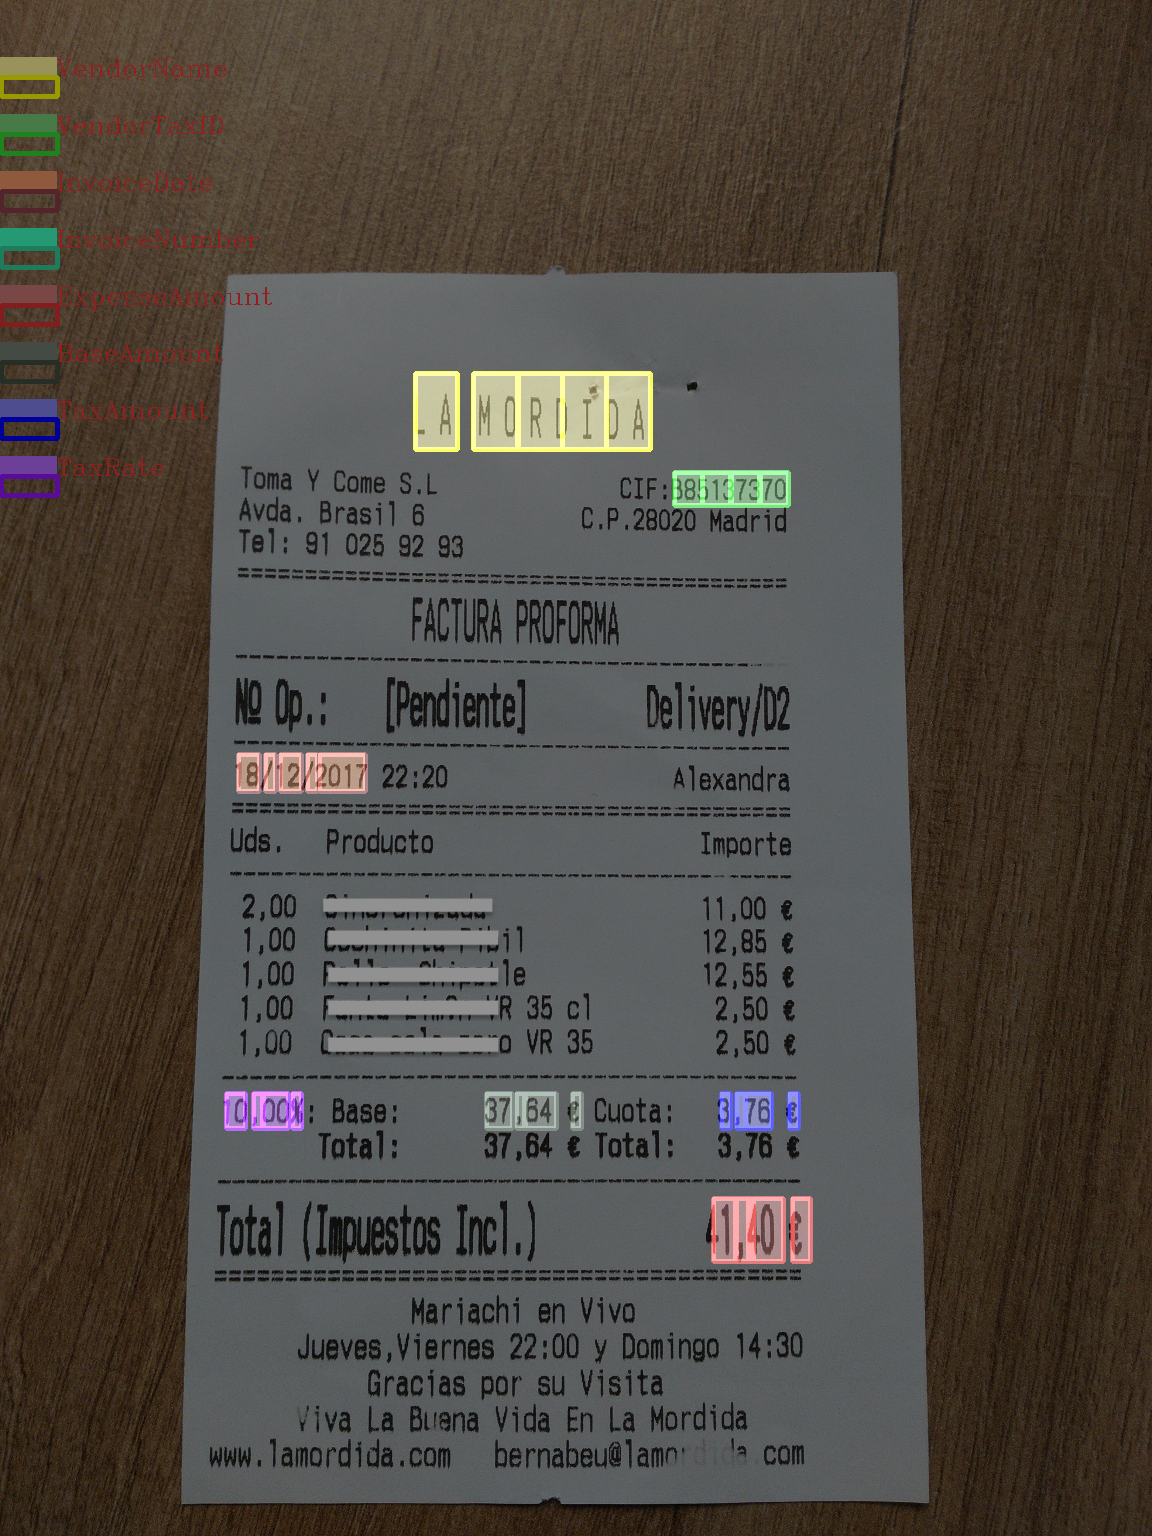
\includegraphics[width=0.19\linewidth]{appendix/meals/Correct_4.png}}  
\subfloat{\fcolorbox{white}{white}{}}
\subfloat{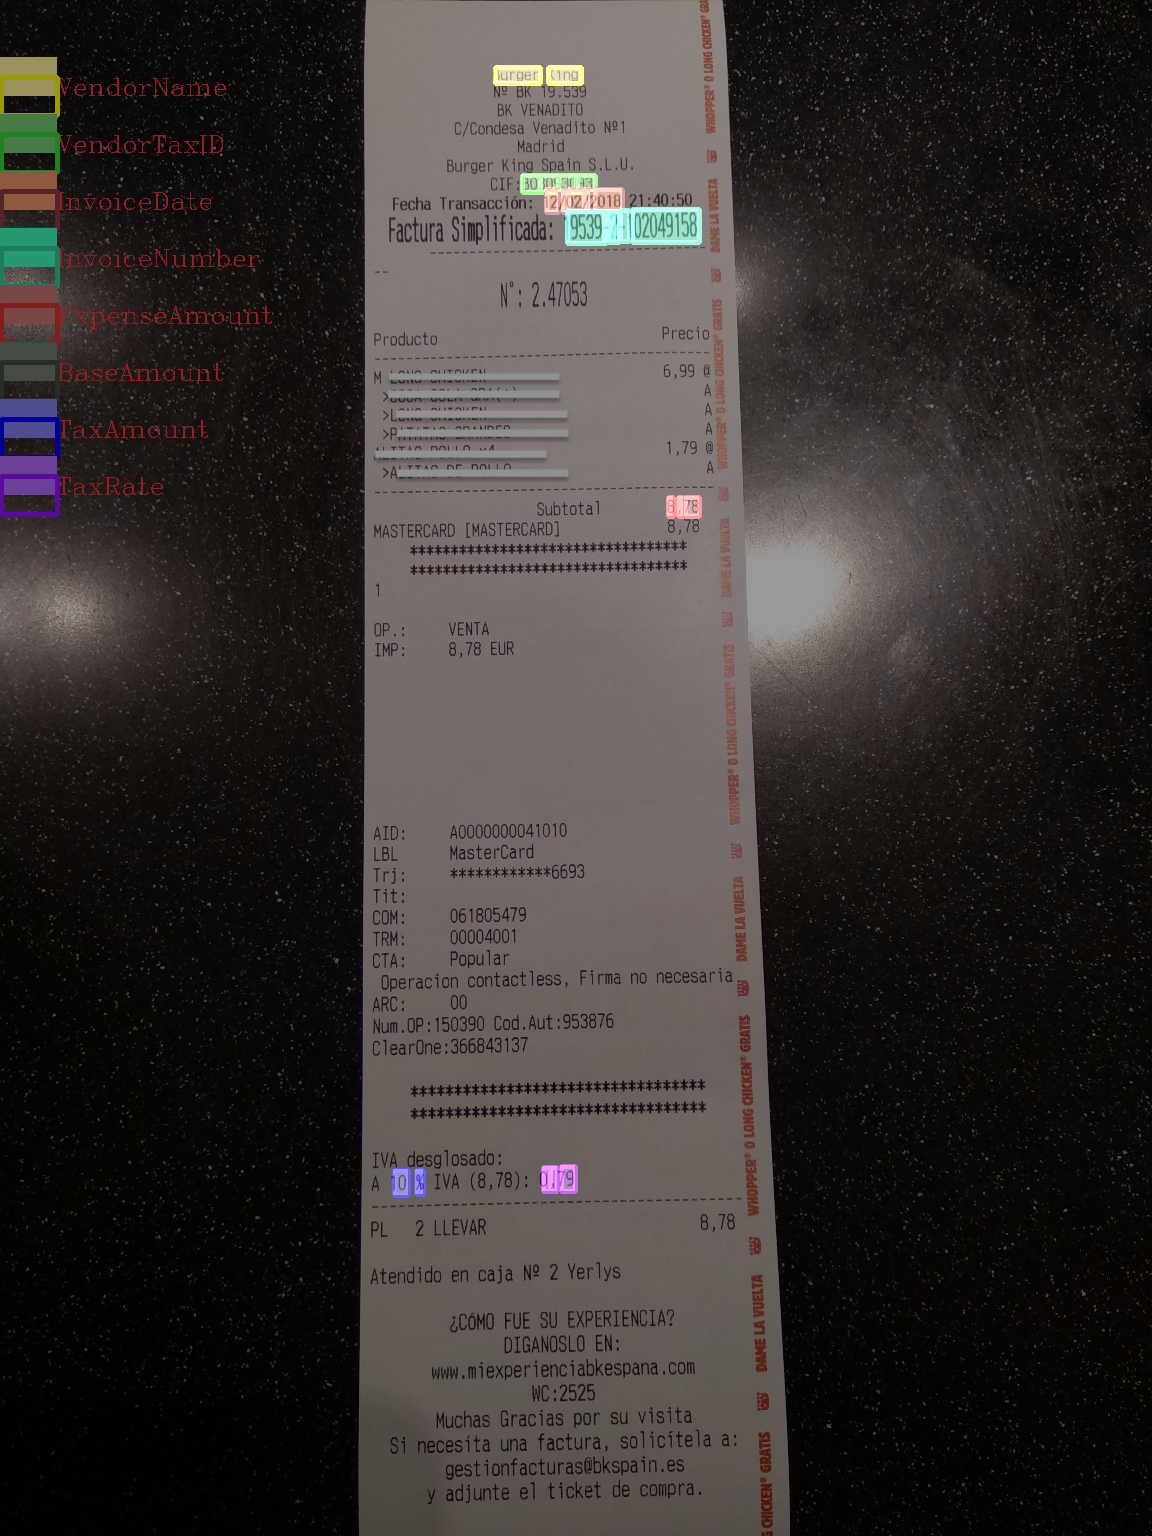
\includegraphics[width=0.19\linewidth]{appendix/meals/Correct_5.png}}  
\subfloat{\fcolorbox{white}{white}{}}
\subfloat{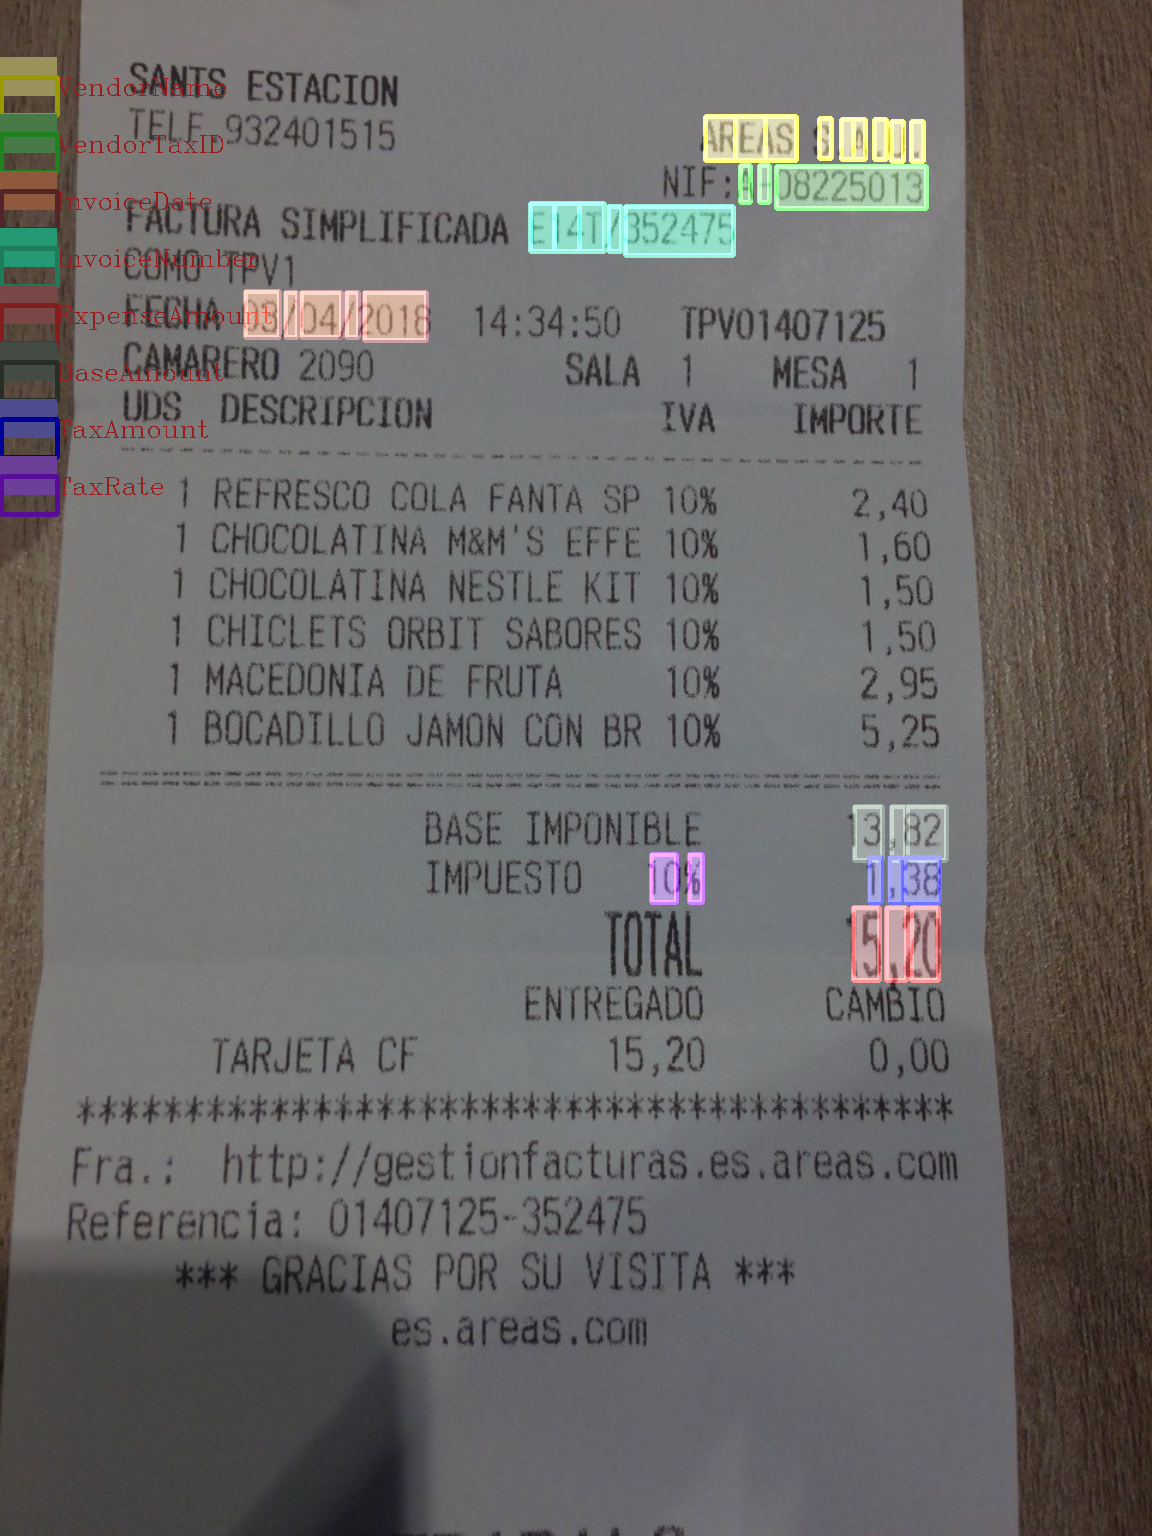
\includegraphics[width=0.19\linewidth]{appendix/meals/Correct_9.png}}  
\subfloat{\fcolorbox{white}{white}{}}
\subfloat{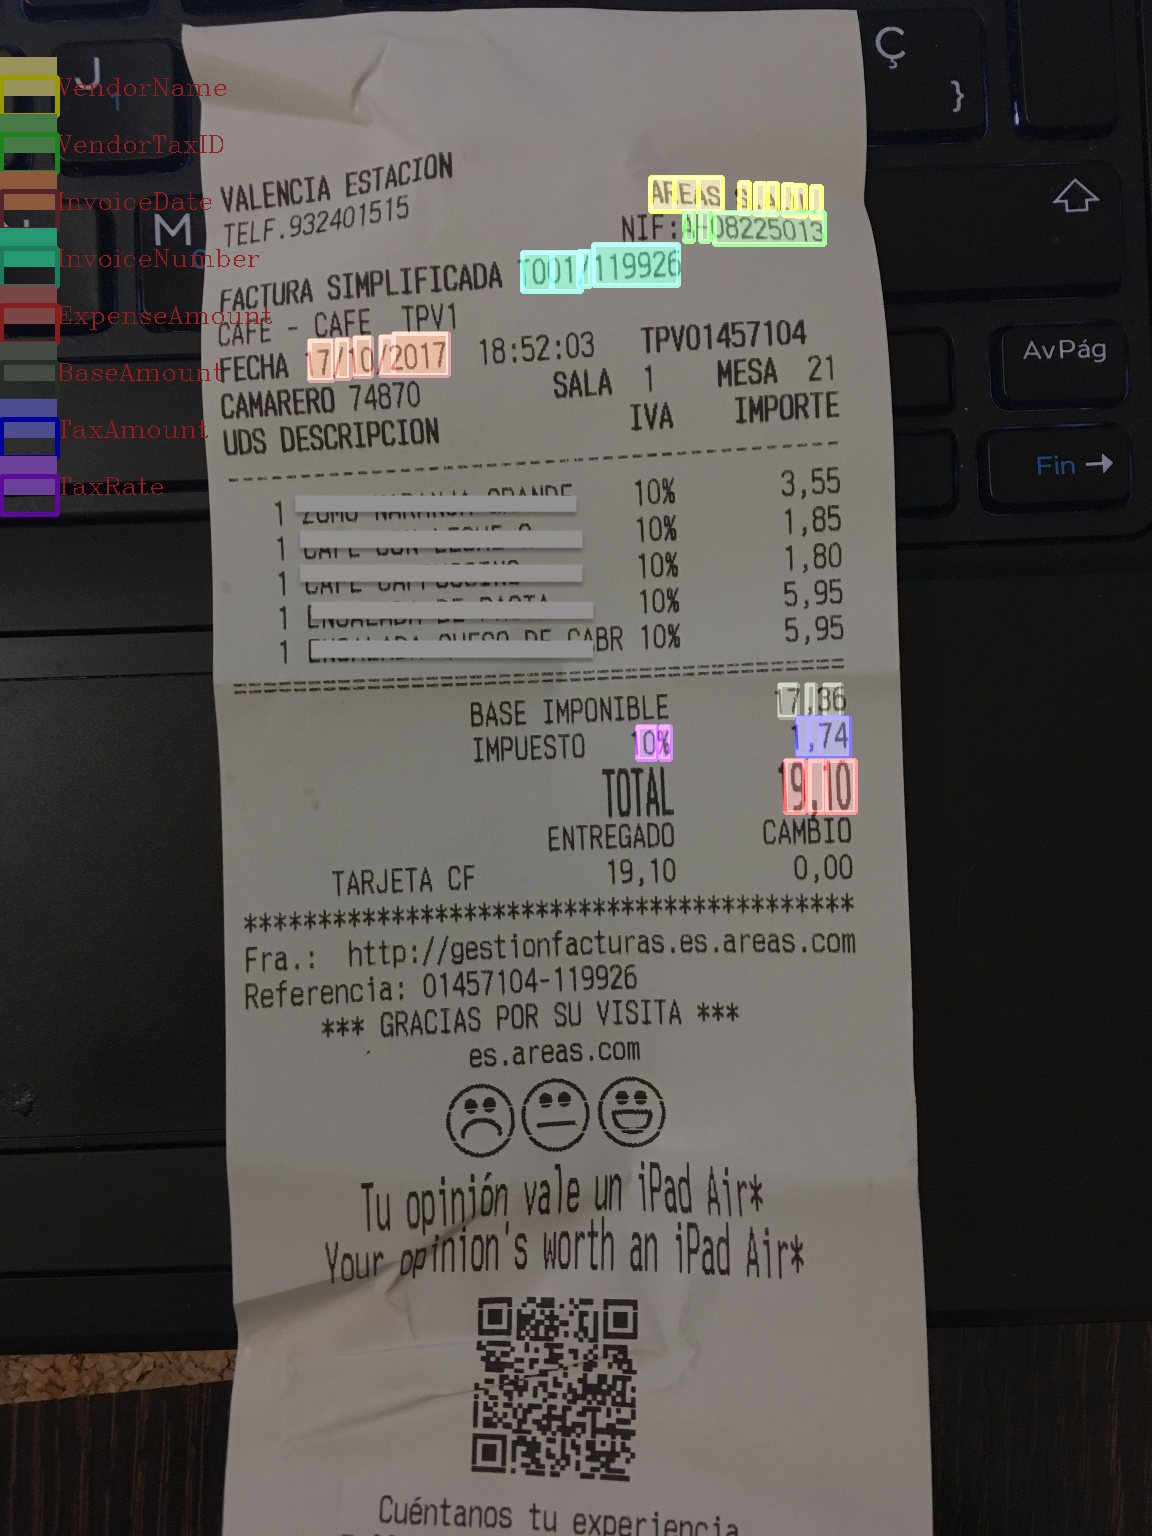
\includegraphics[width=0.19\linewidth]{appendix/meals/Correct_7.png}}  
\subfloat{\fcolorbox{white}{white}{}}
\subfloat{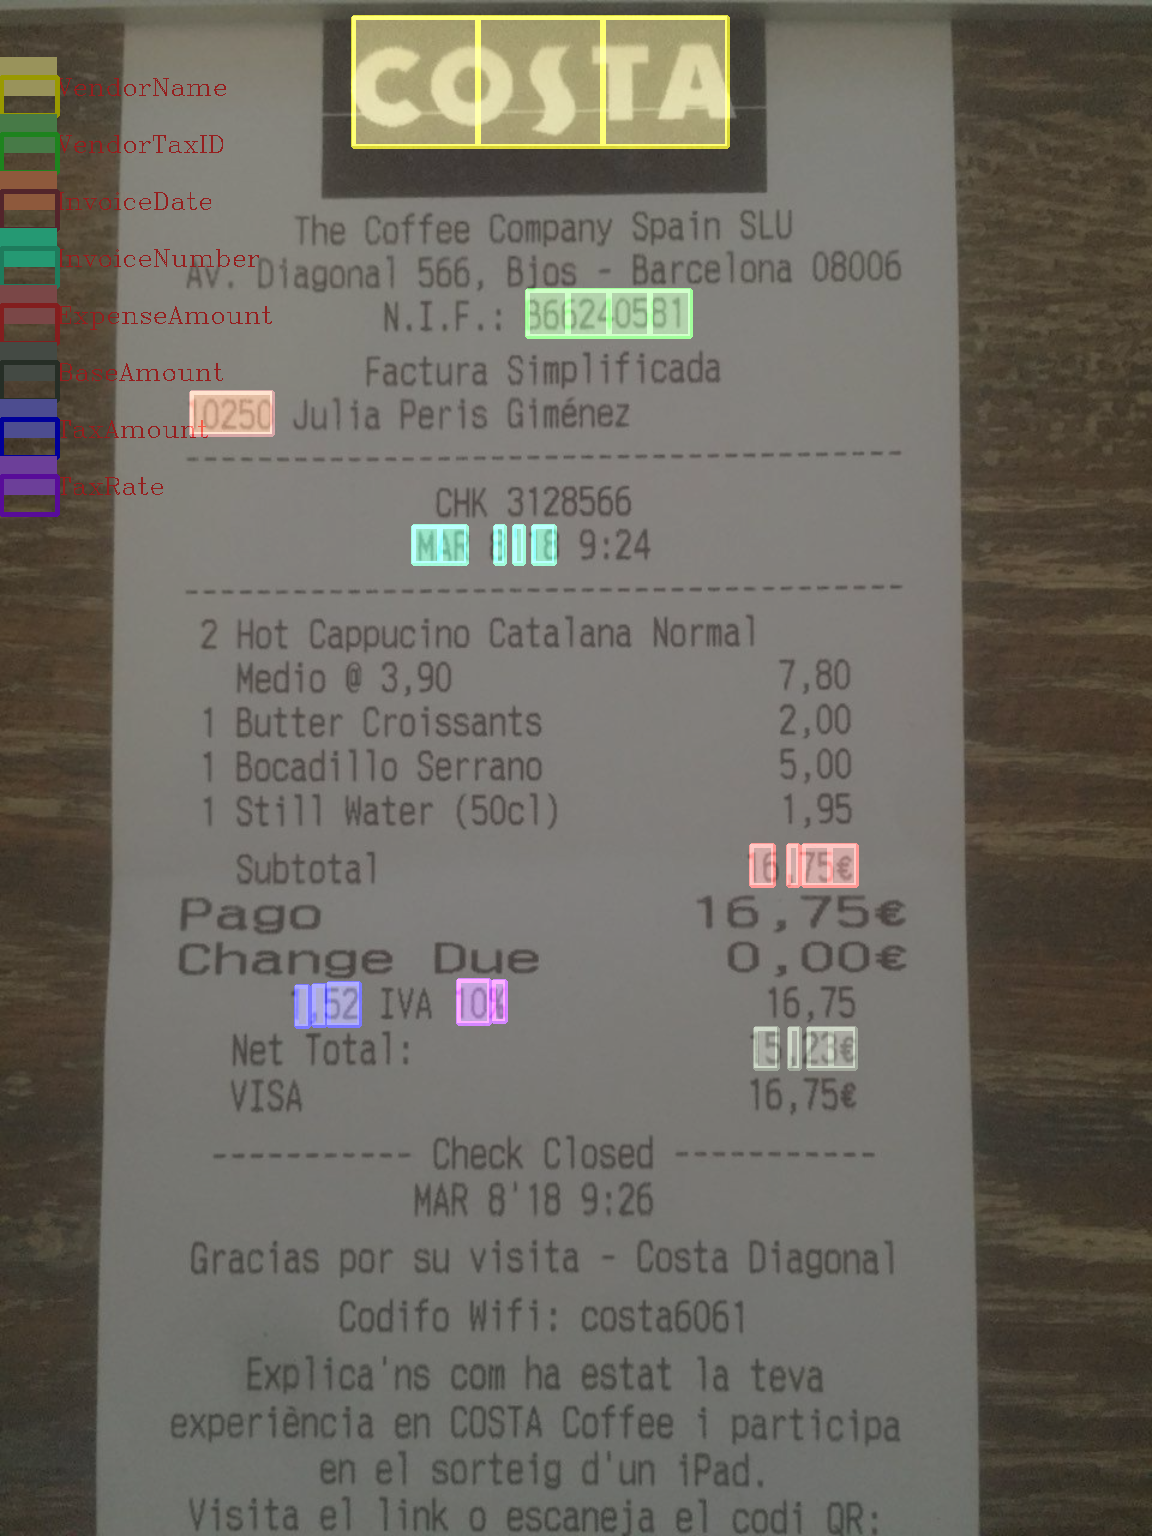
\includegraphics[width=0.19\linewidth]{appendix/meals/Correct_8.png}} \\
\subfloat{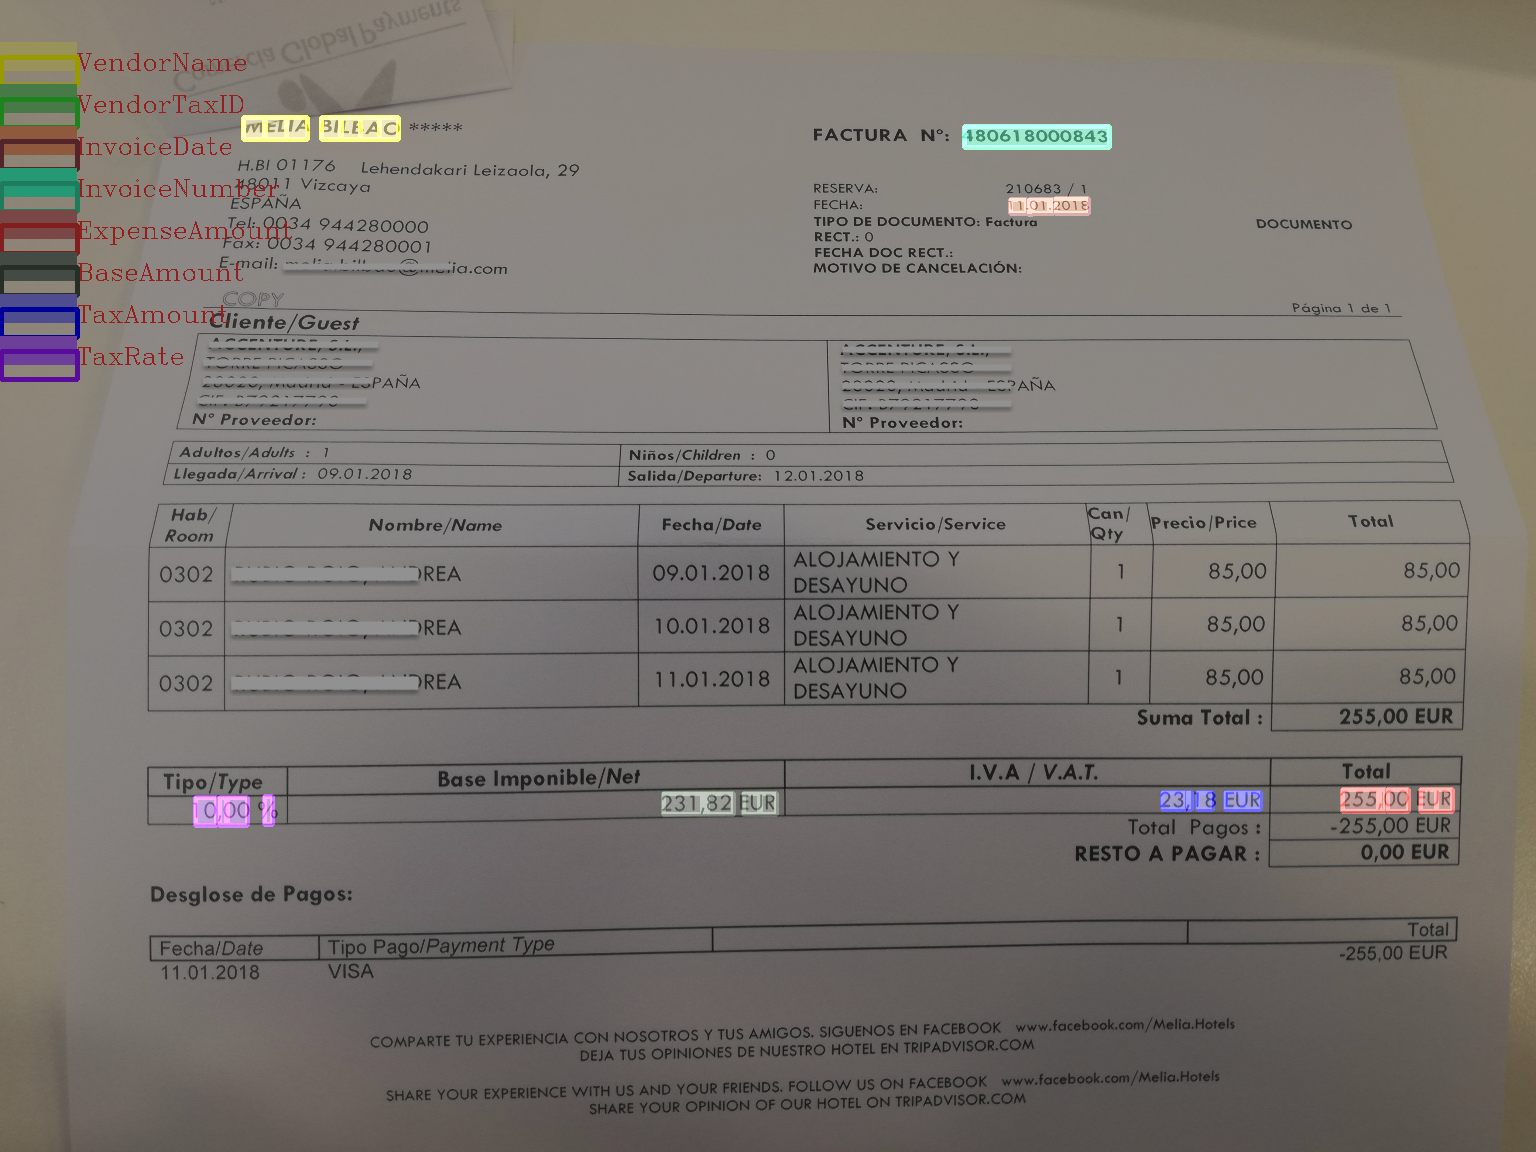
\includegraphics[width=0.35\linewidth]{appendix/hotel/Correct_0.png}}  
\subfloat{\fcolorbox{white}{white}{}}
\subfloat{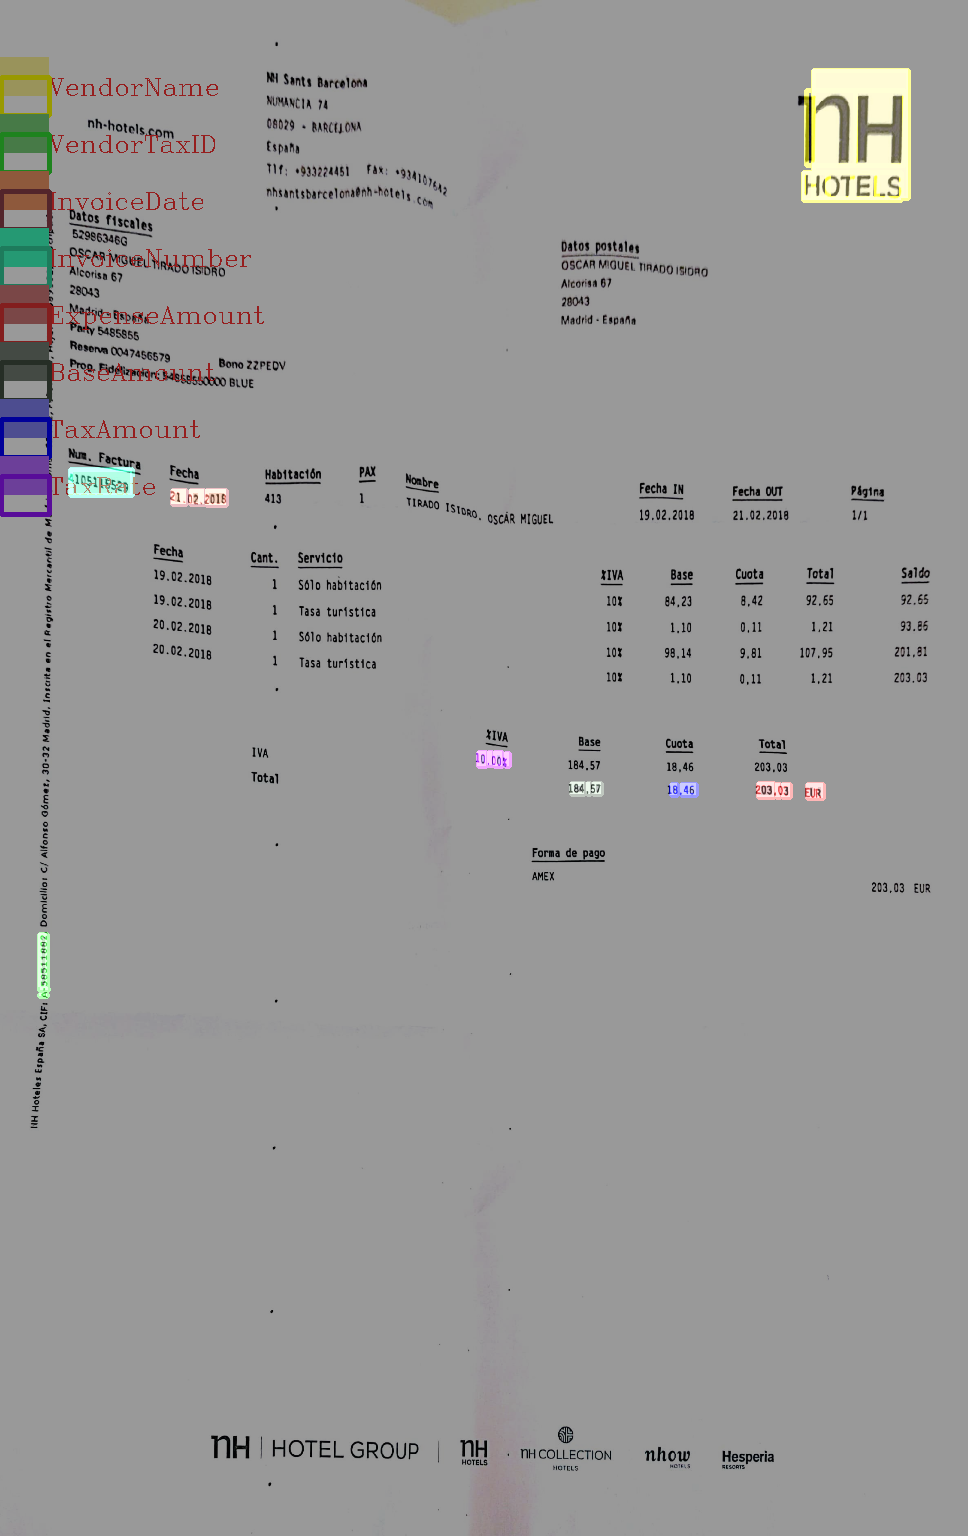
\includegraphics[width=0.19\linewidth]{appendix/hotel/Correct_1.png}}  
\subfloat{\fcolorbox{white}{white}{}}
\subfloat{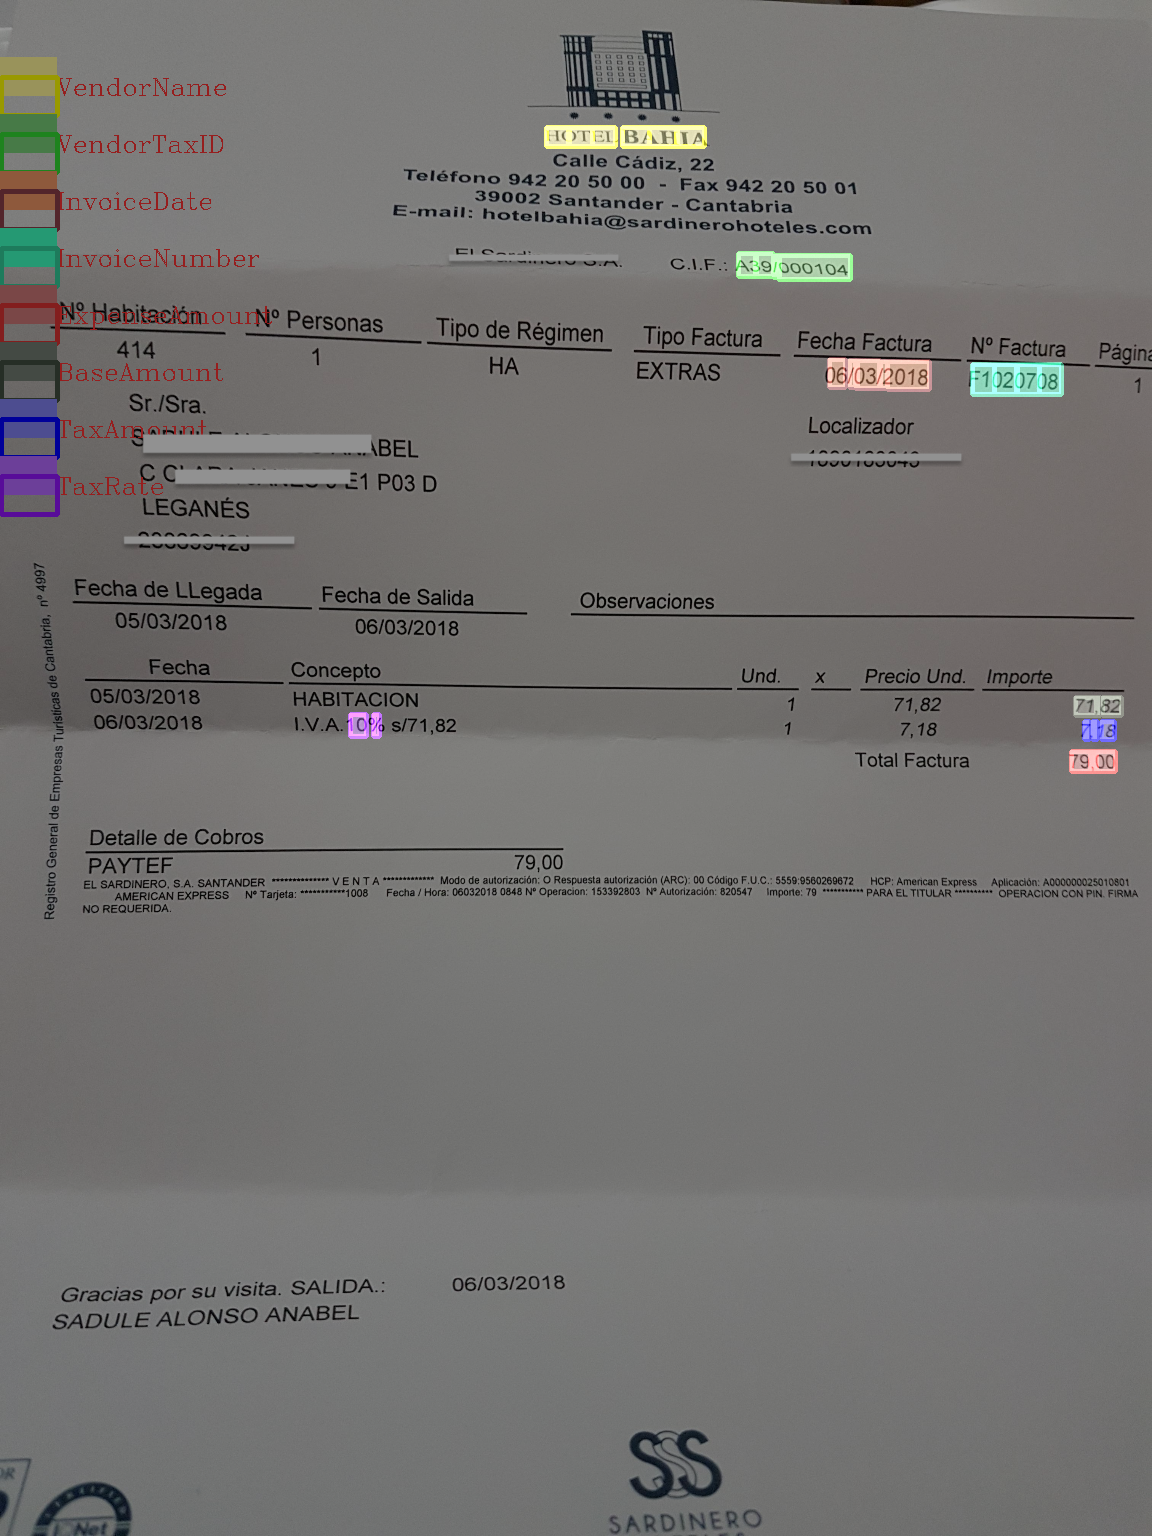
\includegraphics[width=0.21\linewidth]{appendix/hotel/Correct_2.png}}  
\subfloat{\fcolorbox{white}{white}{}}
\subfloat{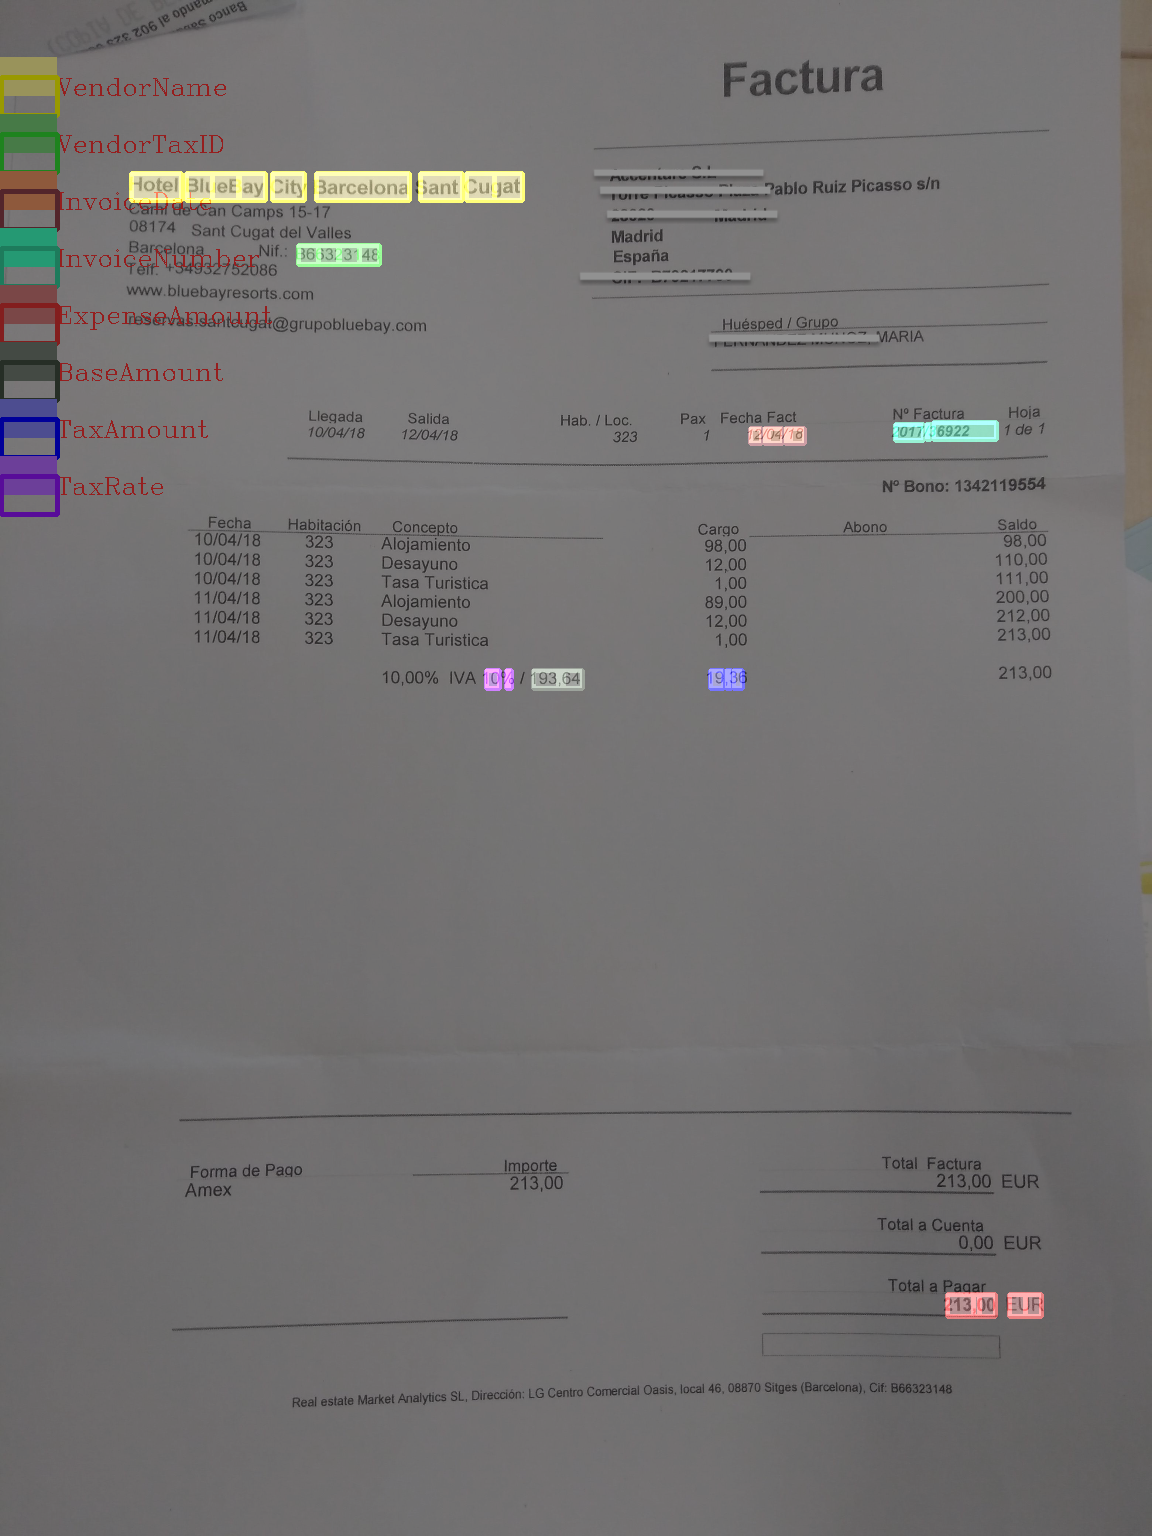
\includegraphics[width=0.21\linewidth]{appendix/hotel/Correct_3.png}}  
\end{center}
   \caption{Example of CUITE inference results. Color legend in the top-left corner indicates the key information classes. Each color indicates a key information class, where filled rectangles are the ground truths while the boundary-only rectangles are the inference results. The result is perfectly correct as if the filled rectangles overlap with the boundary-only rectangles.}
\label{fig:result}
\end{figure*}

Typical examples of receipts with low AP but high softAP score are shown in Figure \ref{fig:falsepositive}. Most of the false positive cases occur in the 'VenderName' class, where names tend to greatly vary and leads to difficulty in model inference. However, it is not hard to find that these false positives can be easily avoided by appending a dictionary based post processor to the key information extractor. One rare false positive case, the third receipt in the first row, is a 'L' letter being mis-recognized as '1' by the employed OCR engine. Although the letter shows distinct appearance from the other digits in the scanned receipt image, it is mis-interpreted as one part of the 'BaseAmount' class due to its close spatial location to the digits and it-self being a digit. It is also can be seen in the first receipt in the second row that several spatial distant digits were wrongly predicted as in the 'BaseAmount' class. Although these are rare cases in our test set, it still suggests that incorporating image-level information may further boost the inference accuracy inspite of the already involved semantical and spatial features. 

\begin{figure}
\begin{center}
\subfloat{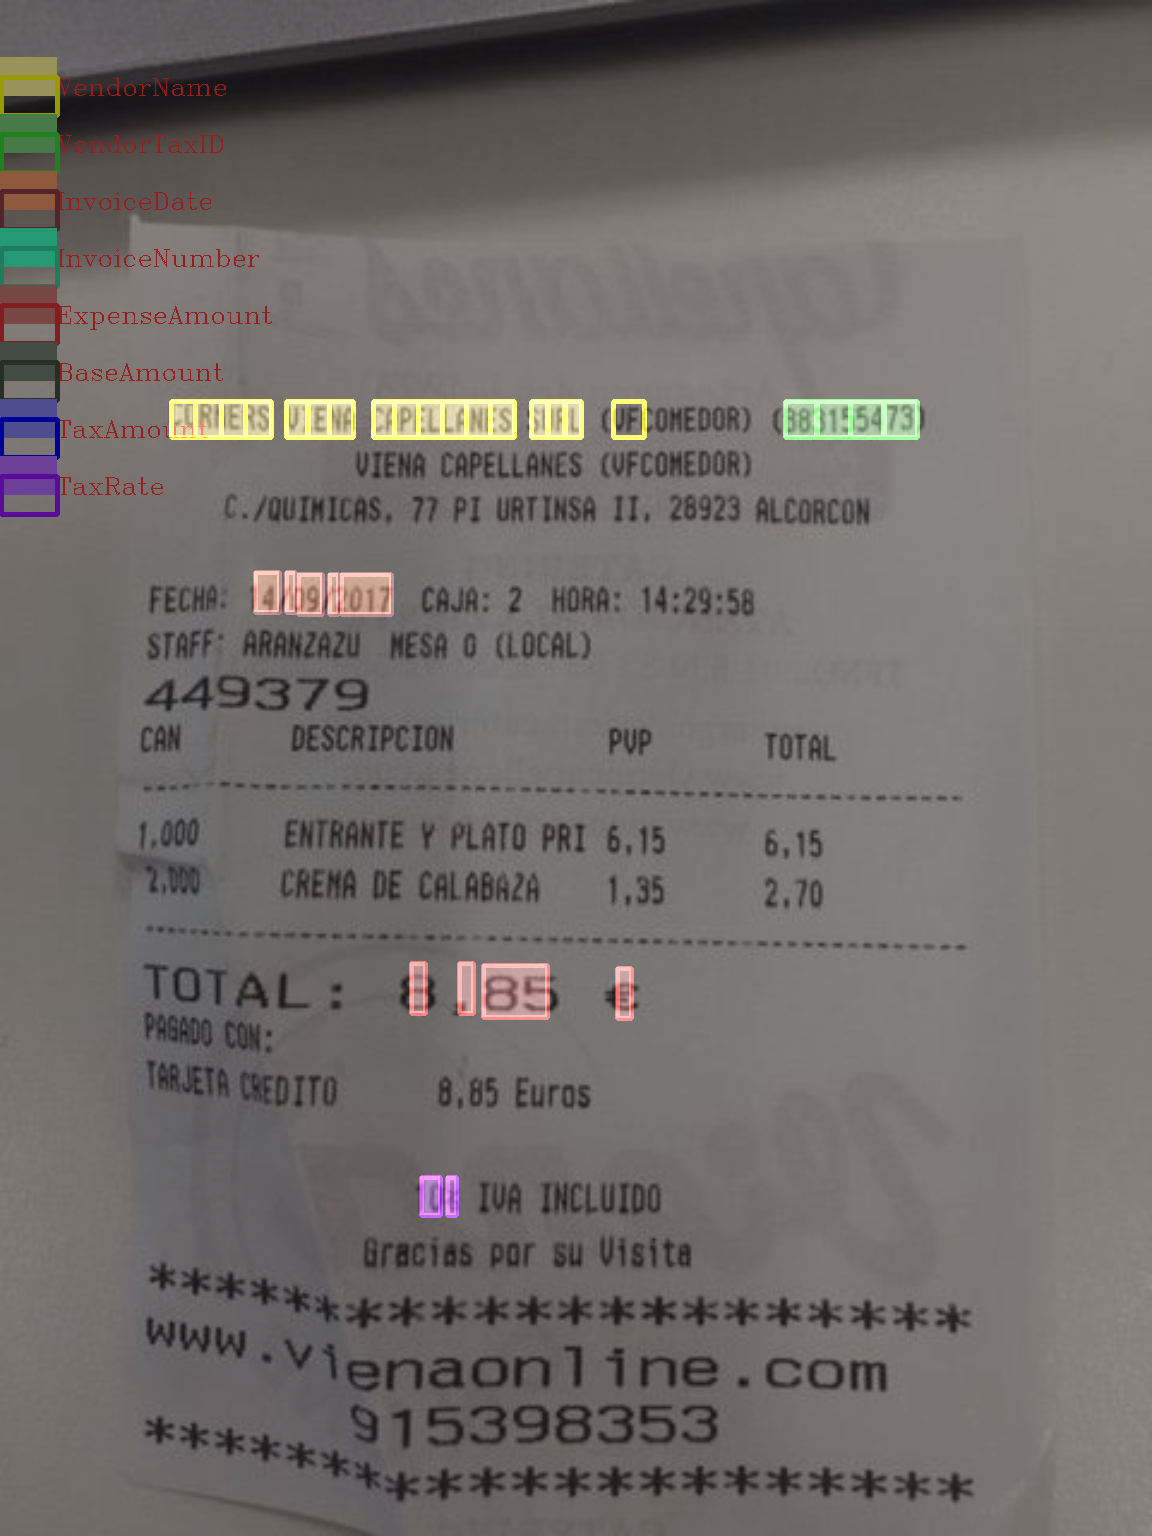
\includegraphics[width=0.31\linewidth]{appendix/meals/FalsePositive_0.png}} 
\subfloat{\fcolorbox{white}{white}{}}
\subfloat{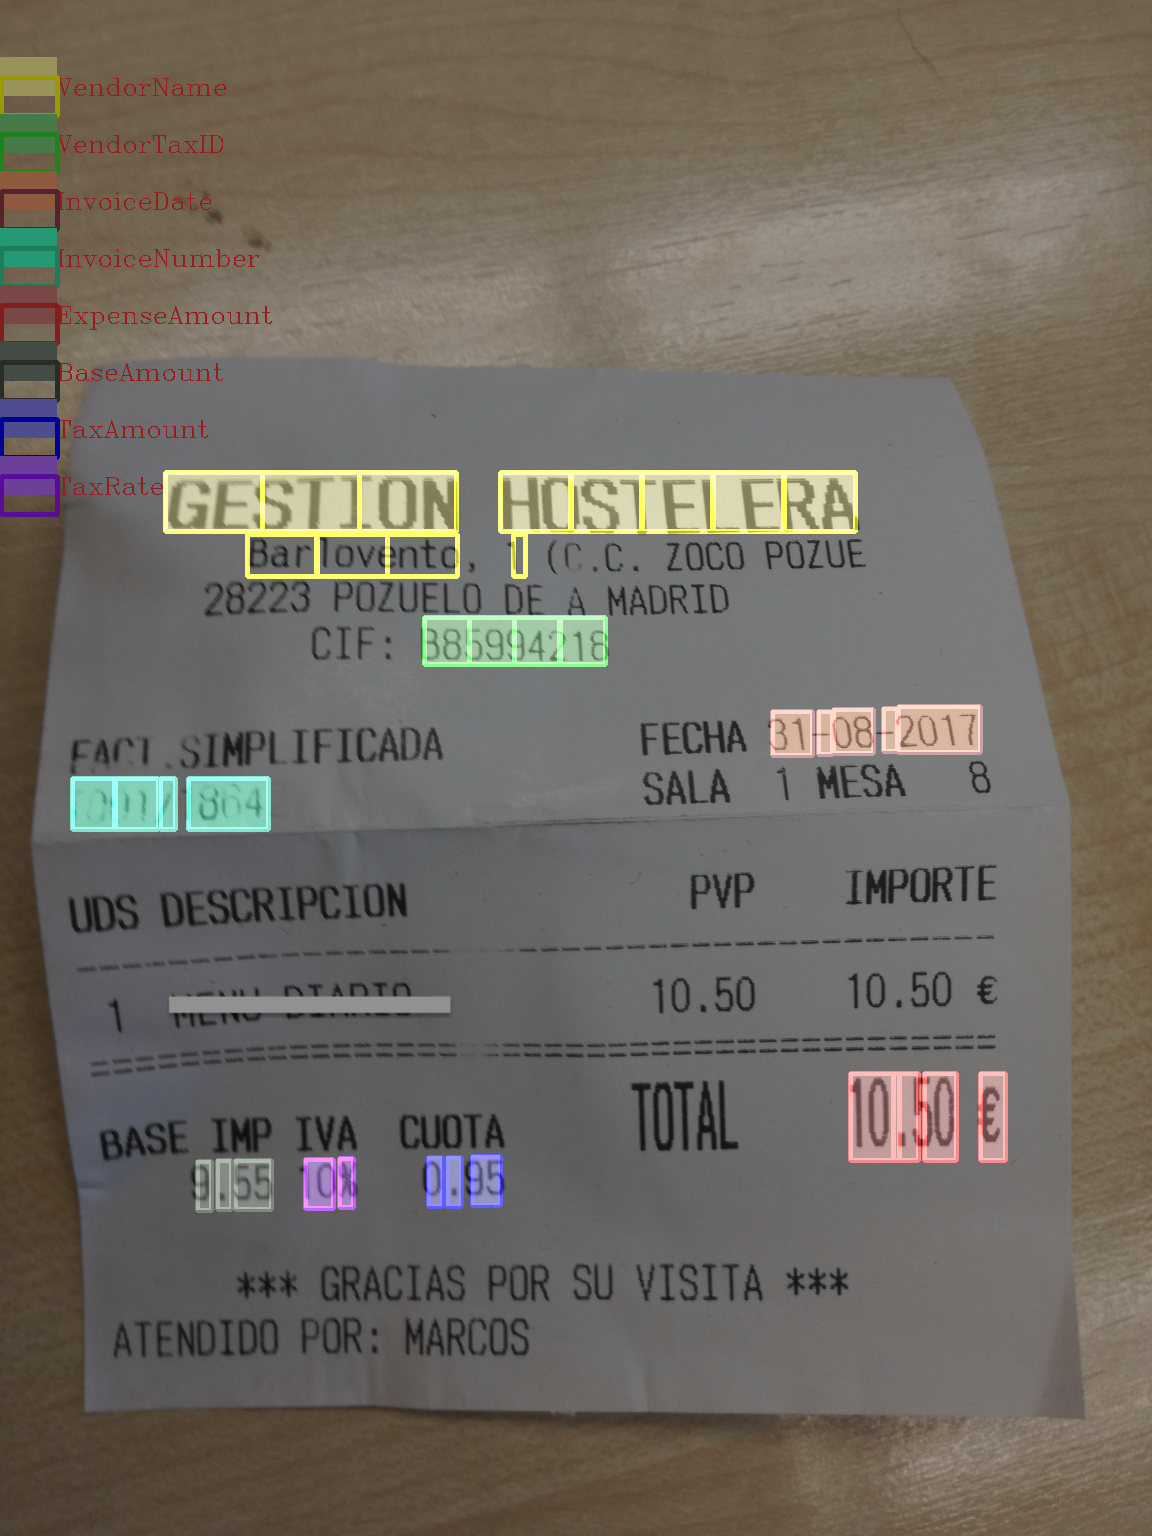
\includegraphics[width=0.31\linewidth]{appendix/meals/FalsePositive_1.png}}
\subfloat{\fcolorbox{white}{white}{}}
\subfloat{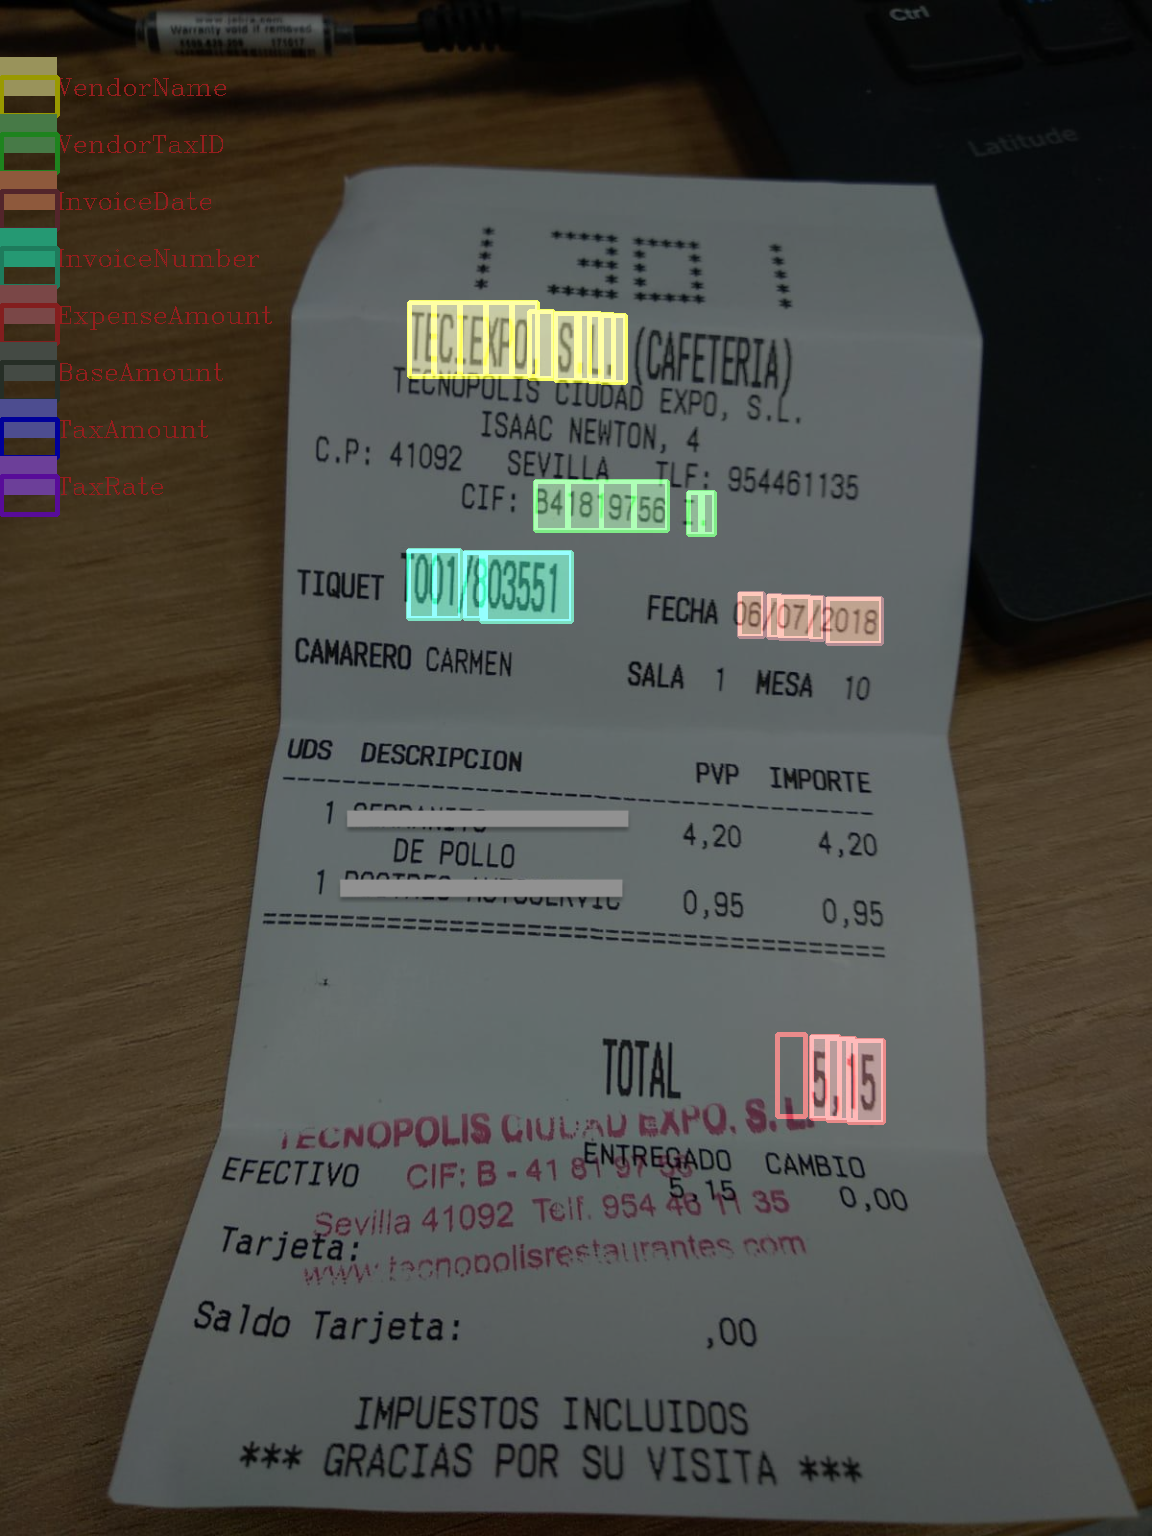
\includegraphics[width=0.31\linewidth]{appendix/meals/FalsePositive_3.png}}\\
\subfloat{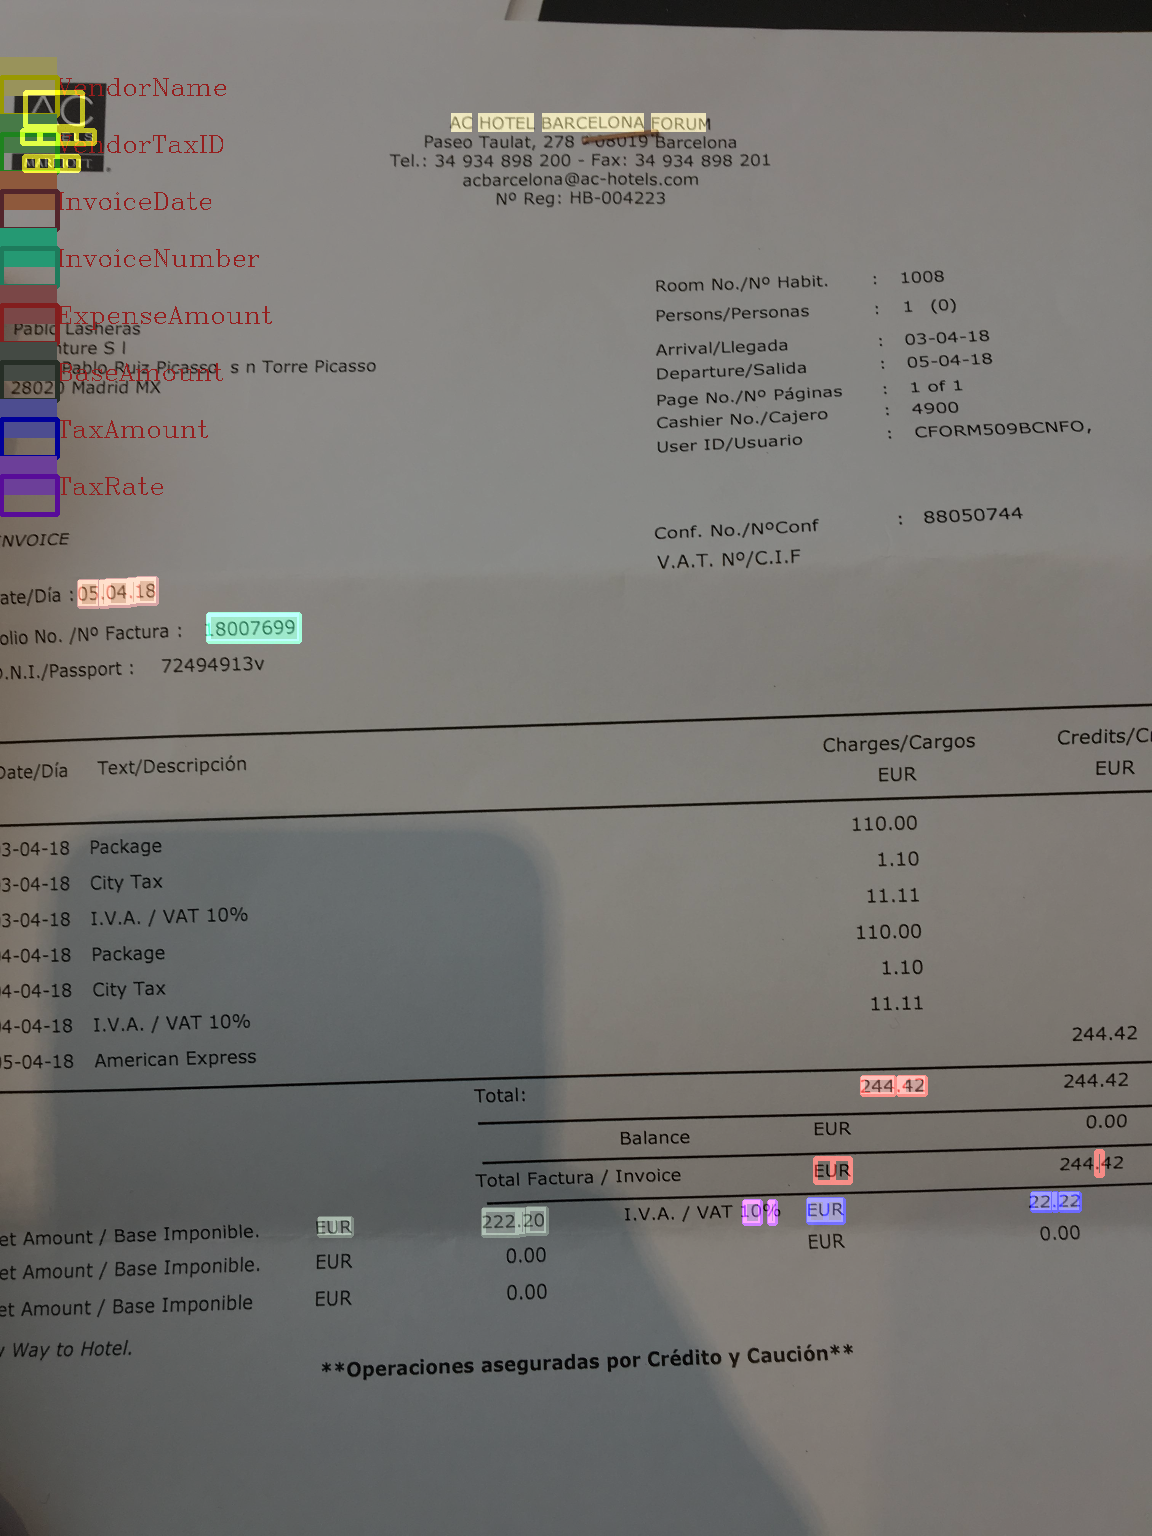
\includegraphics[width=0.29\linewidth]{appendix/hotel/FalsePositive_0.png}}
\subfloat{\fcolorbox{white}{white}{}}
\subfloat{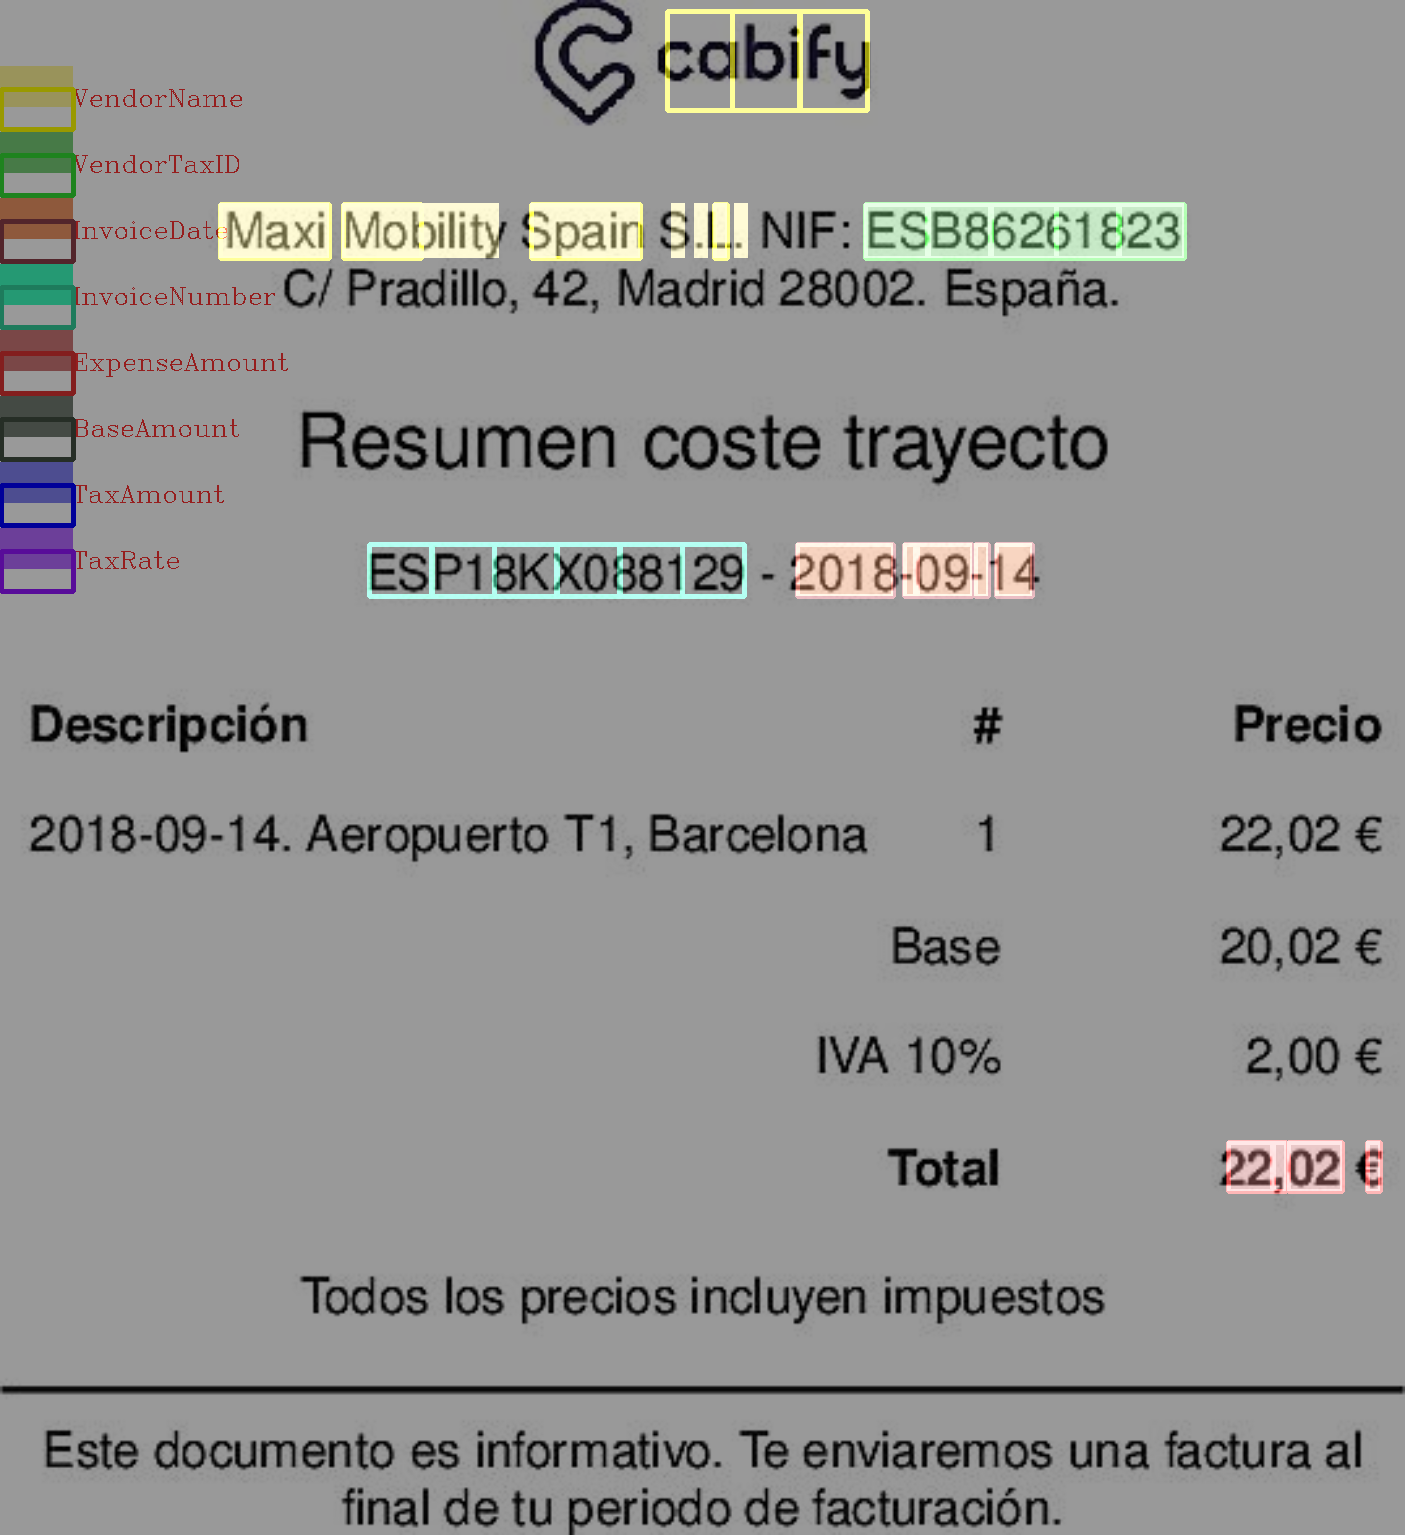
\includegraphics[width=0.35\linewidth]{appendix/taxi/FalsePositive_0.png}}
\subfloat{\fcolorbox{white}{white}{}}
\subfloat{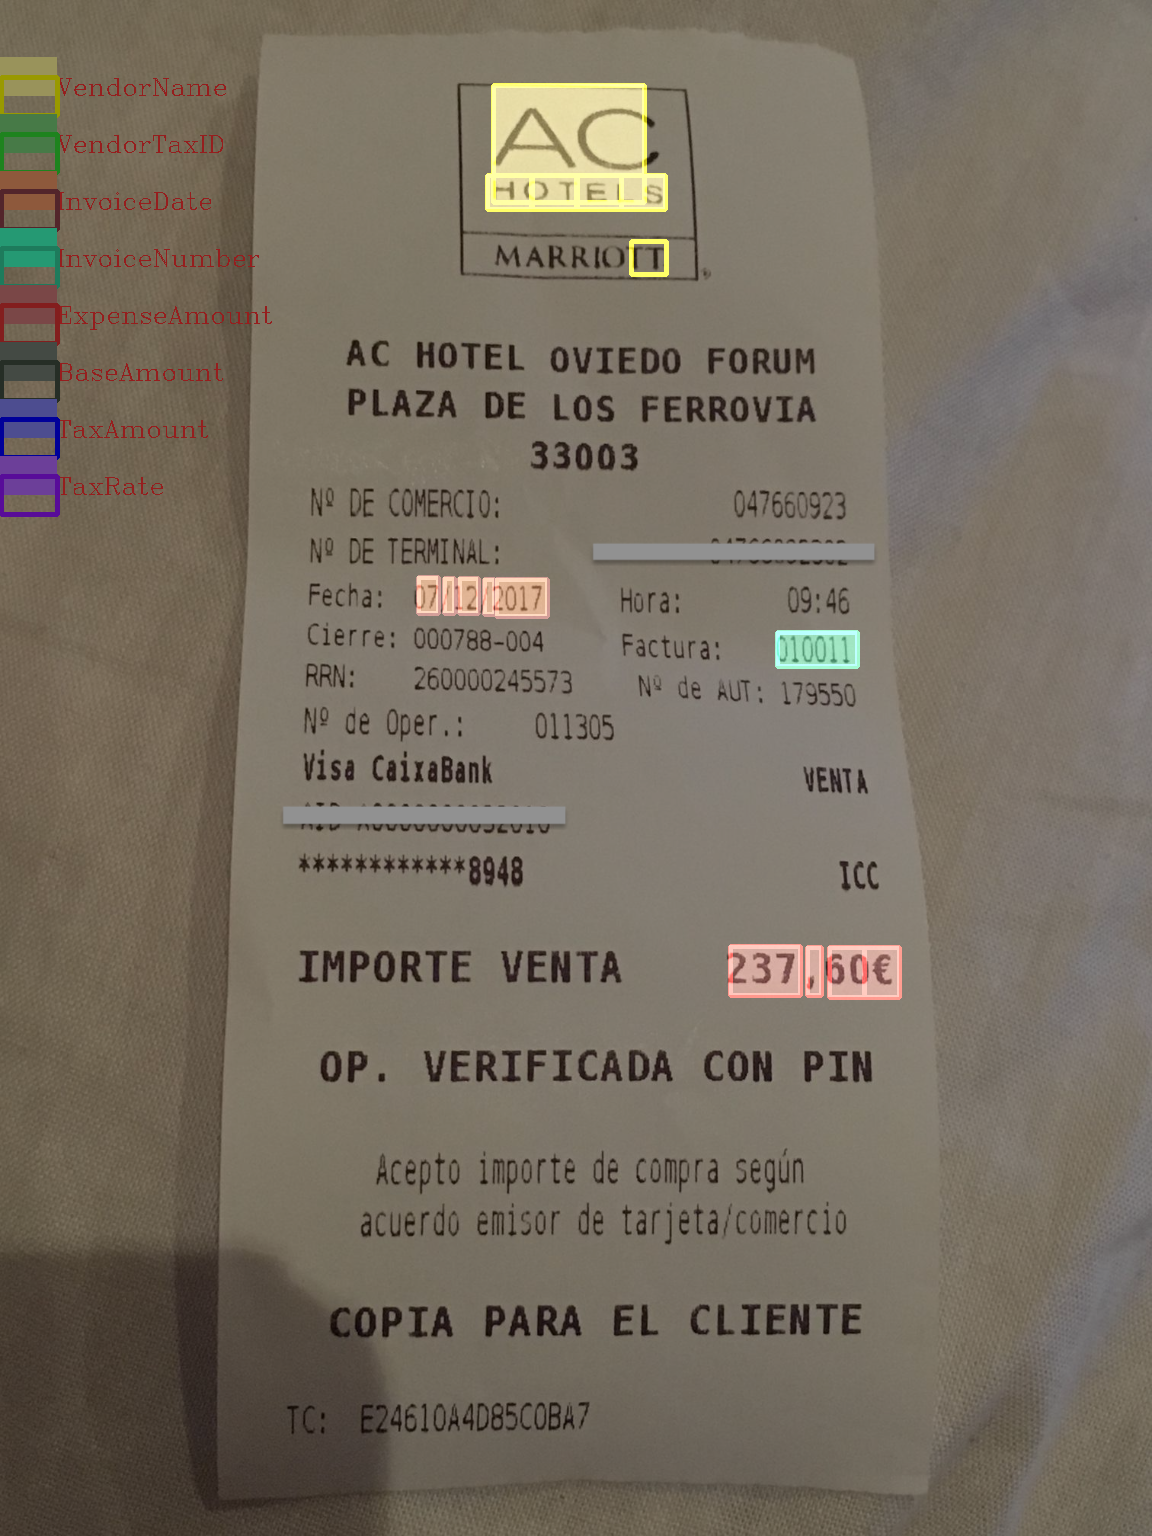
\includegraphics[width=0.29\linewidth]{appendix/hotel/FalsePositive_1.png}}
\subfloat{\fcolorbox{white}{white}{}}
\end{center}
   \caption{False positive examples of CUITE prediction results. Color legend in the top-left corner indicates the key information classes. Each color indicates a key information class, where filled rectangles are the ground truths while the boundary-only rectangles are the inference results. The false positives are results with the boundary-only rectangles being not overlapped with the filled rectangles.}
\label{fig:falsepositive}
\end{figure}

Furthermore, we find that some wrong cases are actually correct since the ground truth were wrongly labelled by the human labelers. As illustrated in Figure \ref{fig:falselabel}, the 'VendorName' appears twice in the scanned image but only being labelled once in both the first and second receipt in the first row, while the model correctly interprets both occurance as the 'VendorName' in the first receipt and correctly interprets the second occurance in the second receipt. Furthermore, 'TaxRate' is neglected to be labeled in the third receipt in the first row and 'VendorName' is wrongly labelled in the first receipt in the second row. The third receipt in the second row and the first and second receipt in the third row are all neglected with labelling 'TaxRate', and the third receipt in the third row is neglected with labelling 'BaseAmount' while the trained model correctly inferred the right class. It is not hard to find that the trained model produces even better results than human labeler on these receipts, which further proves the effectiveness of the proposed method.
\begin{figure}
\begin{center}
\subfloat{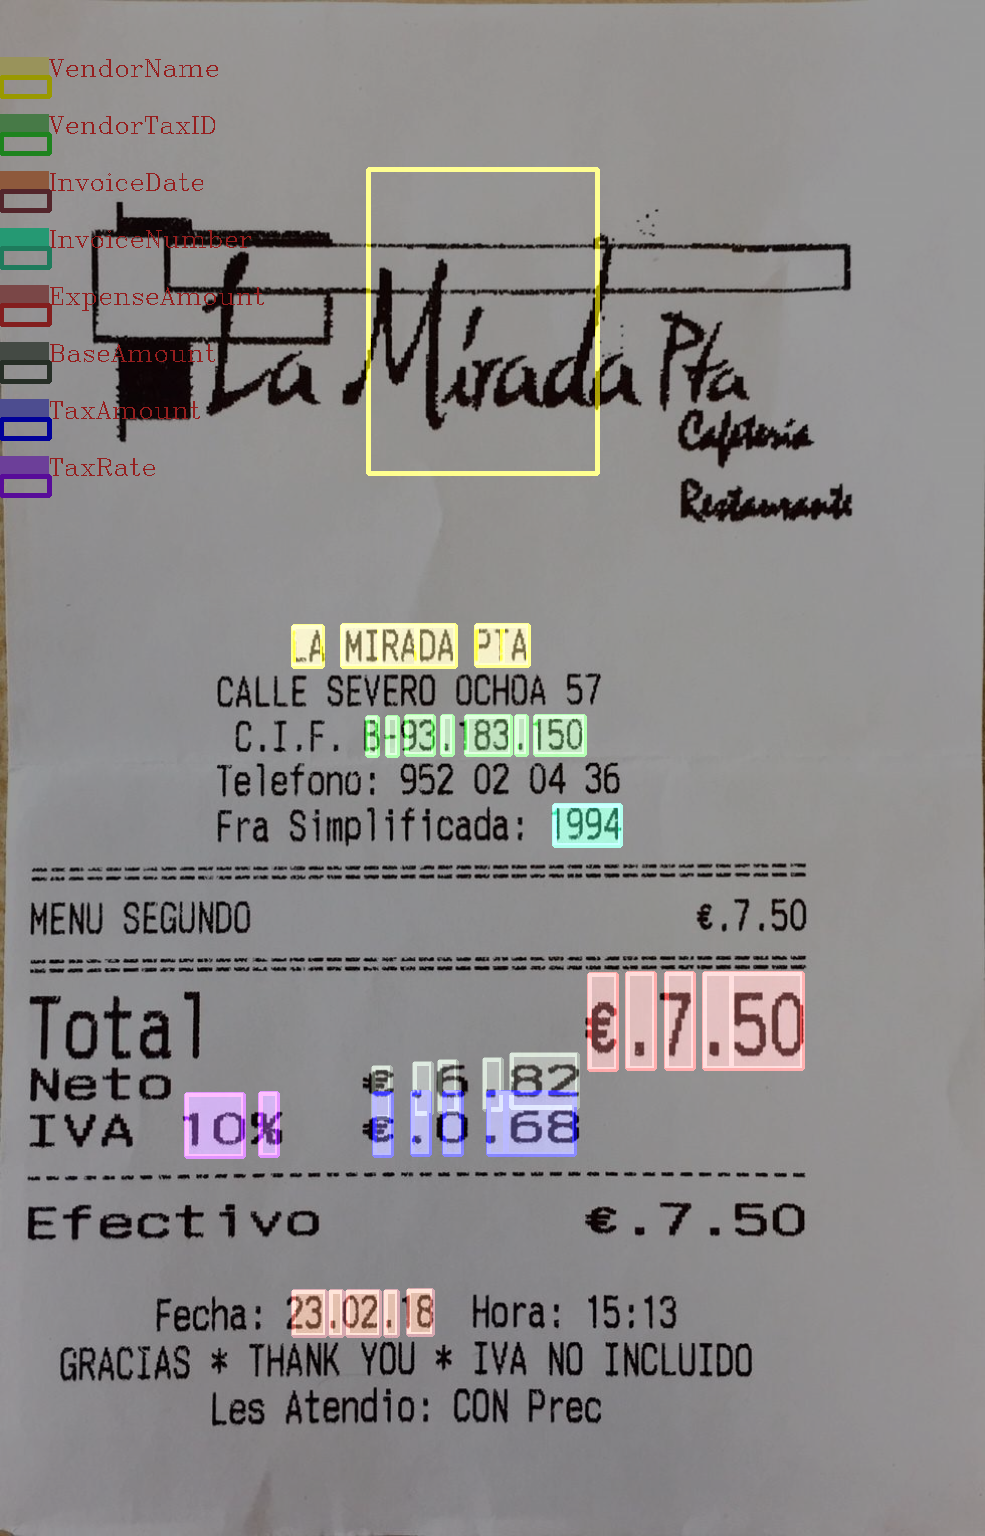
\includegraphics[width=0.28\linewidth]{appendix/meals/FalseLabel_0.png}} 
\subfloat{\fcolorbox{white}{white}{}}
\subfloat{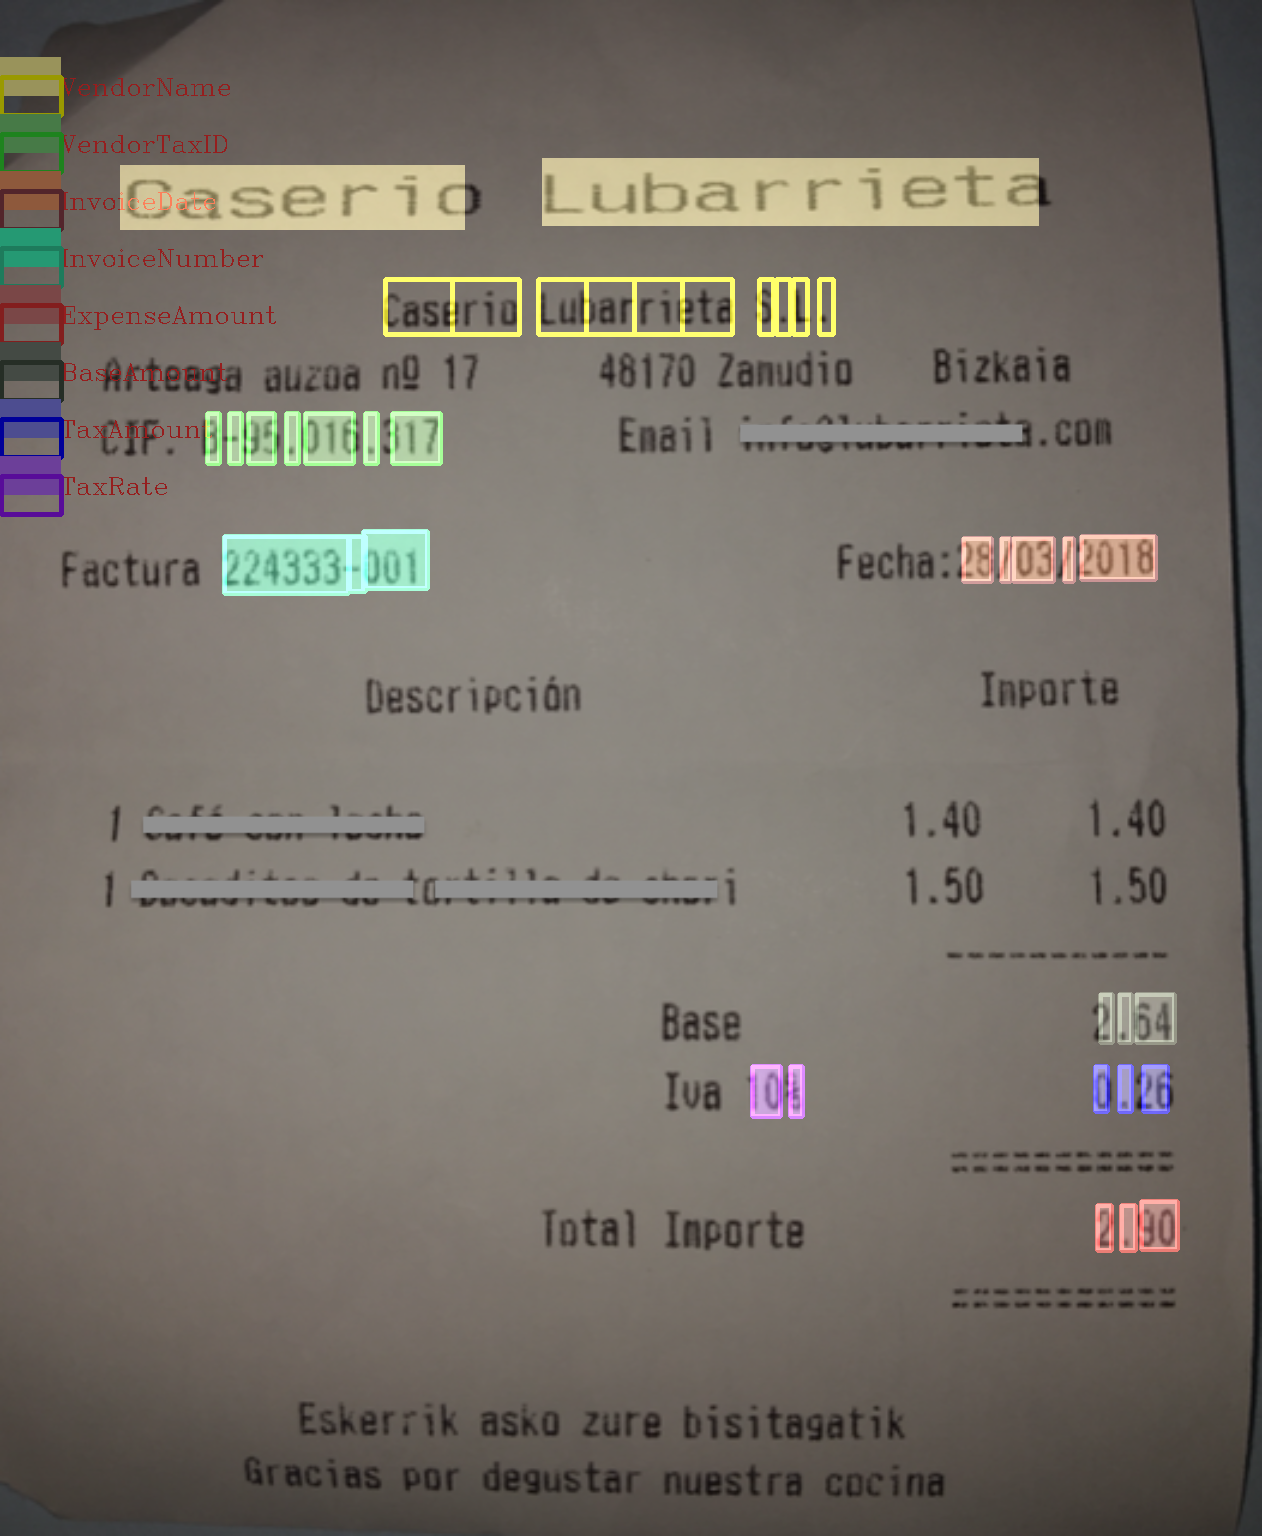
\includegraphics[width=0.34\linewidth]{appendix/meals/FalseLabel_1.png}} 
\subfloat{\fcolorbox{white}{white}{}}
\subfloat{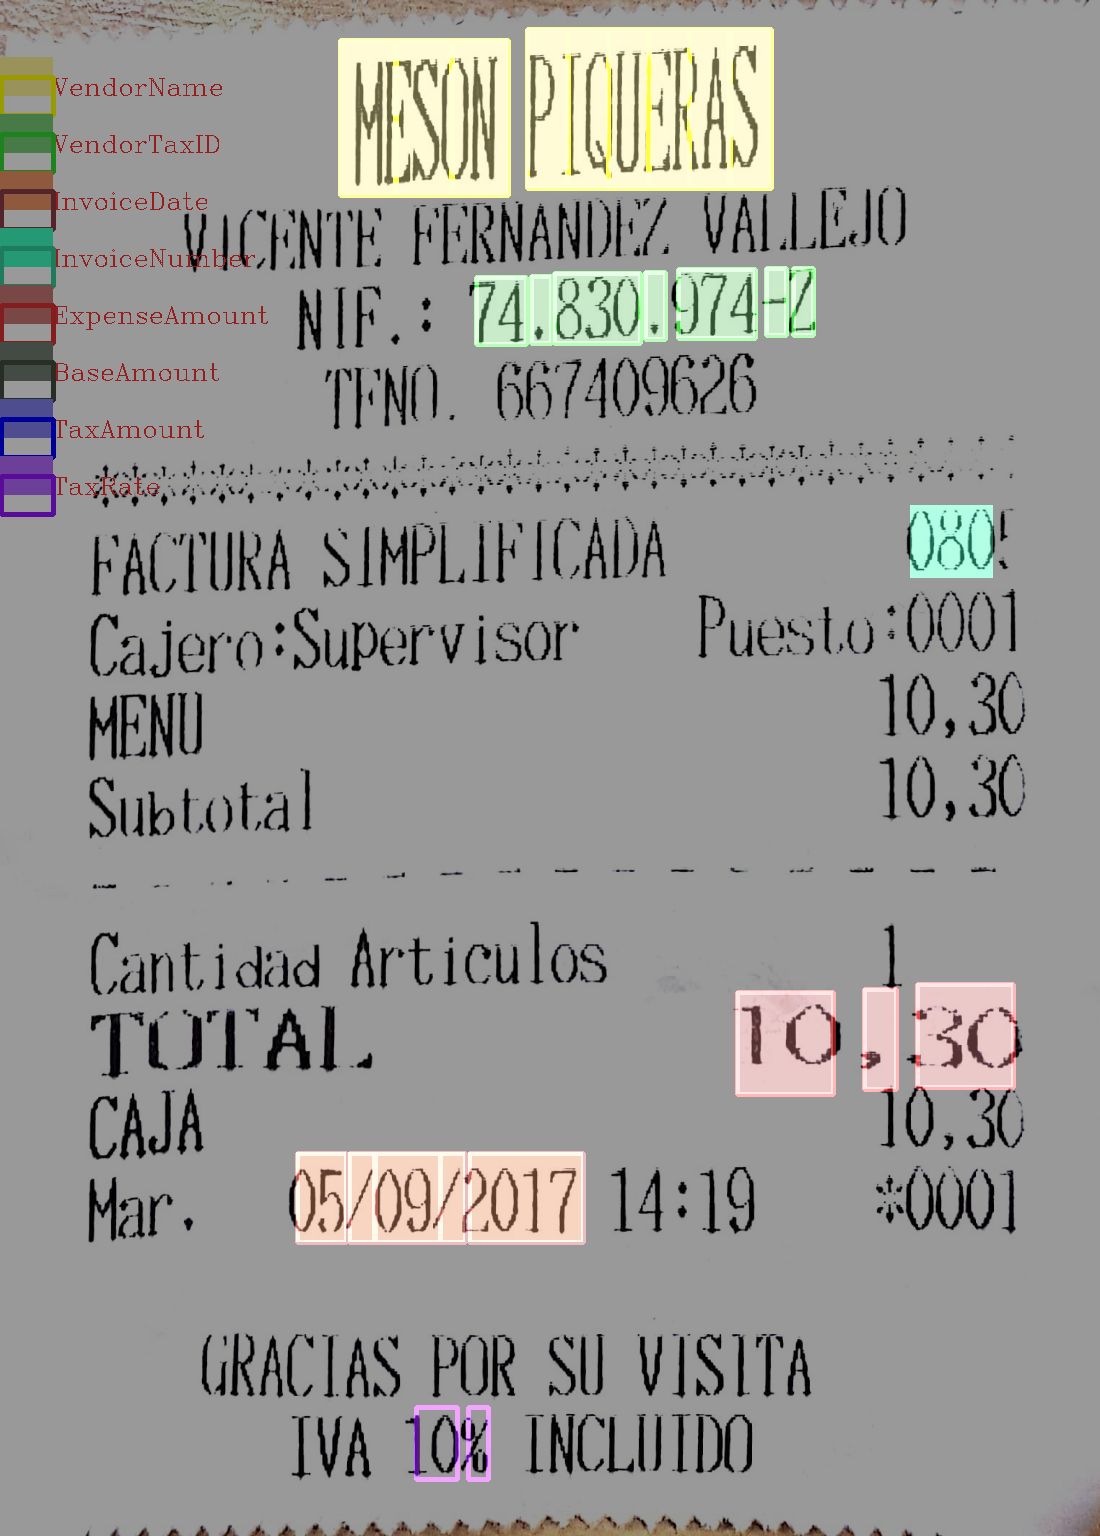
\includegraphics[width=0.31\linewidth]{appendix/meals/FalseLabel_2.png}}\\
\subfloat{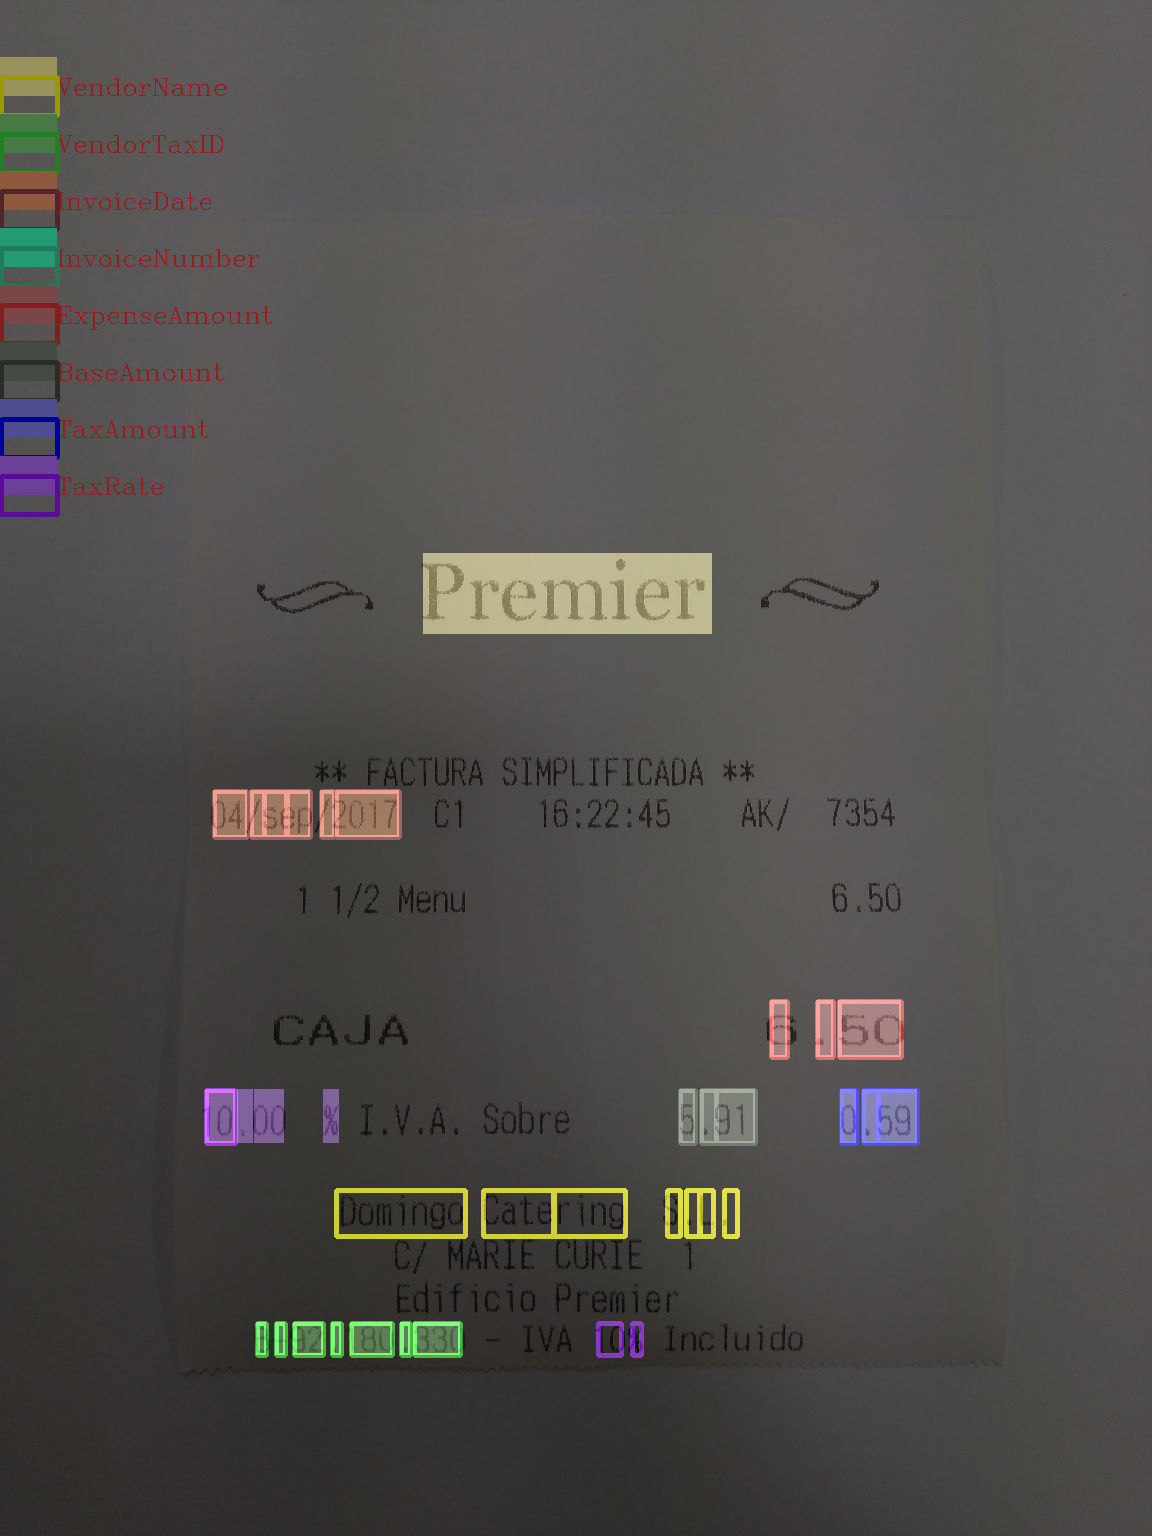
\includegraphics[width=0.31\linewidth]{appendix/meals/FalseLabel_3.png}} 
\subfloat{\fcolorbox{white}{white}{}}
\subfloat{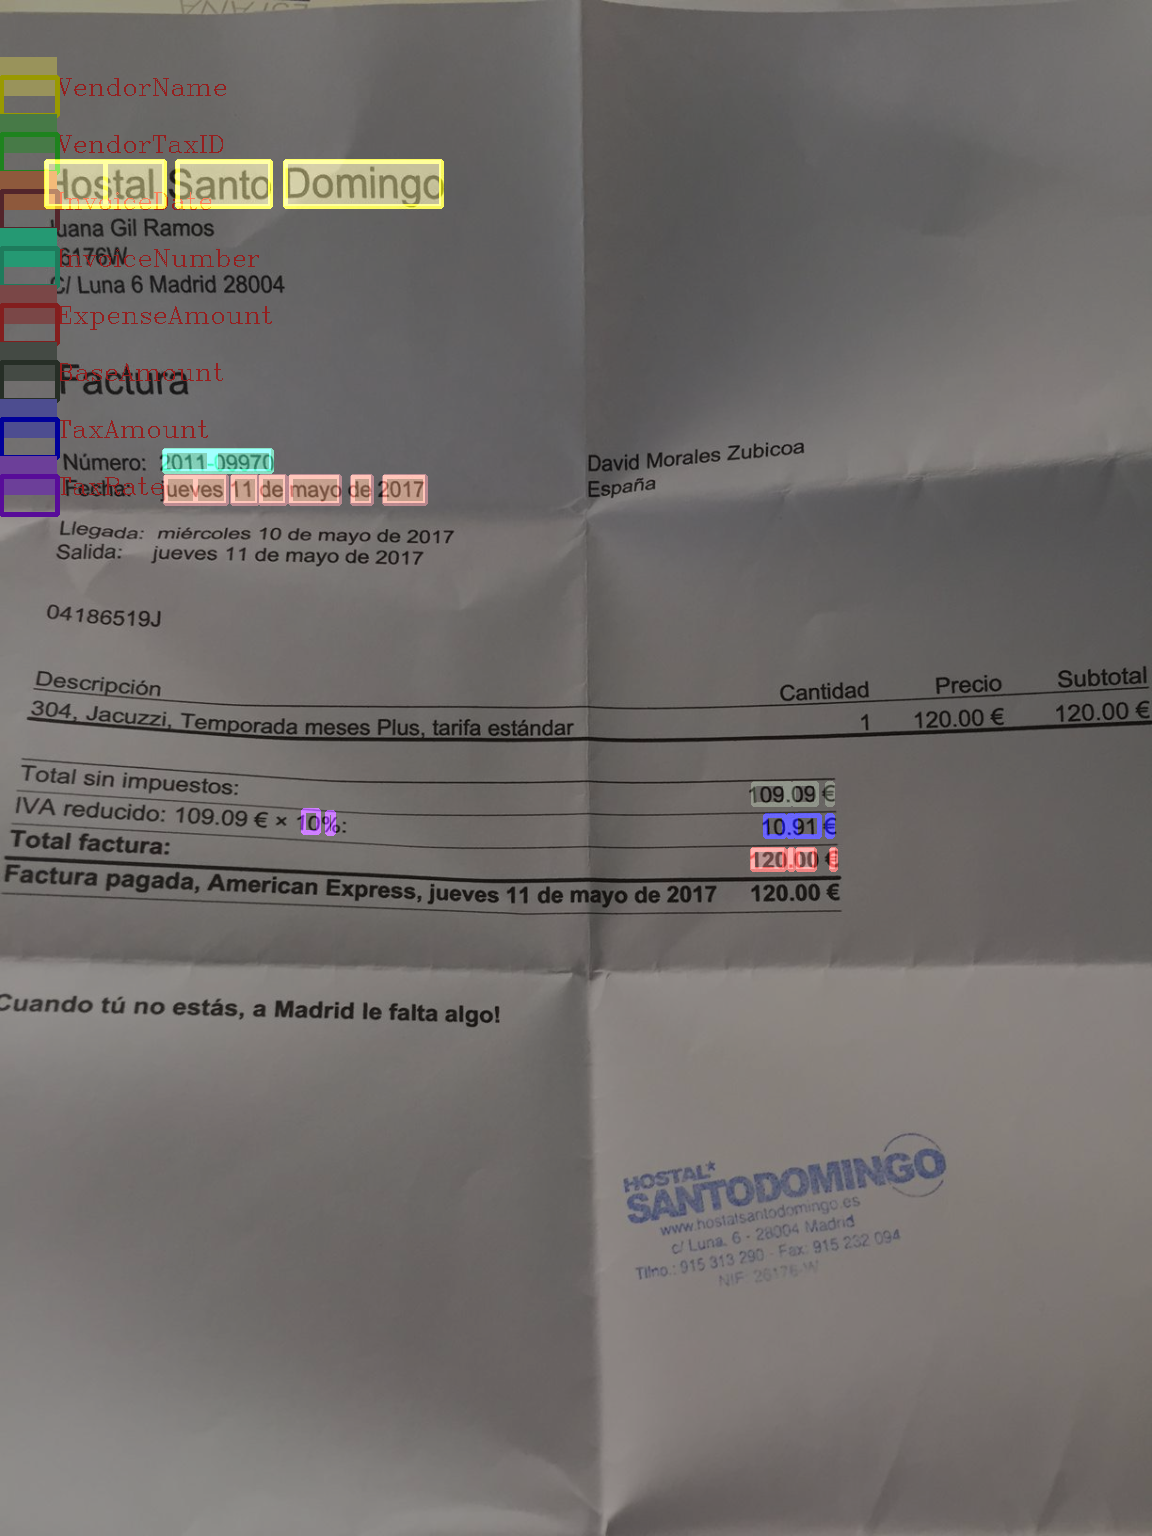
\includegraphics[width=0.31\linewidth]{appendix/hotel/FalseLabel_0.png}}
\subfloat{\fcolorbox{white}{white}{}}
\subfloat{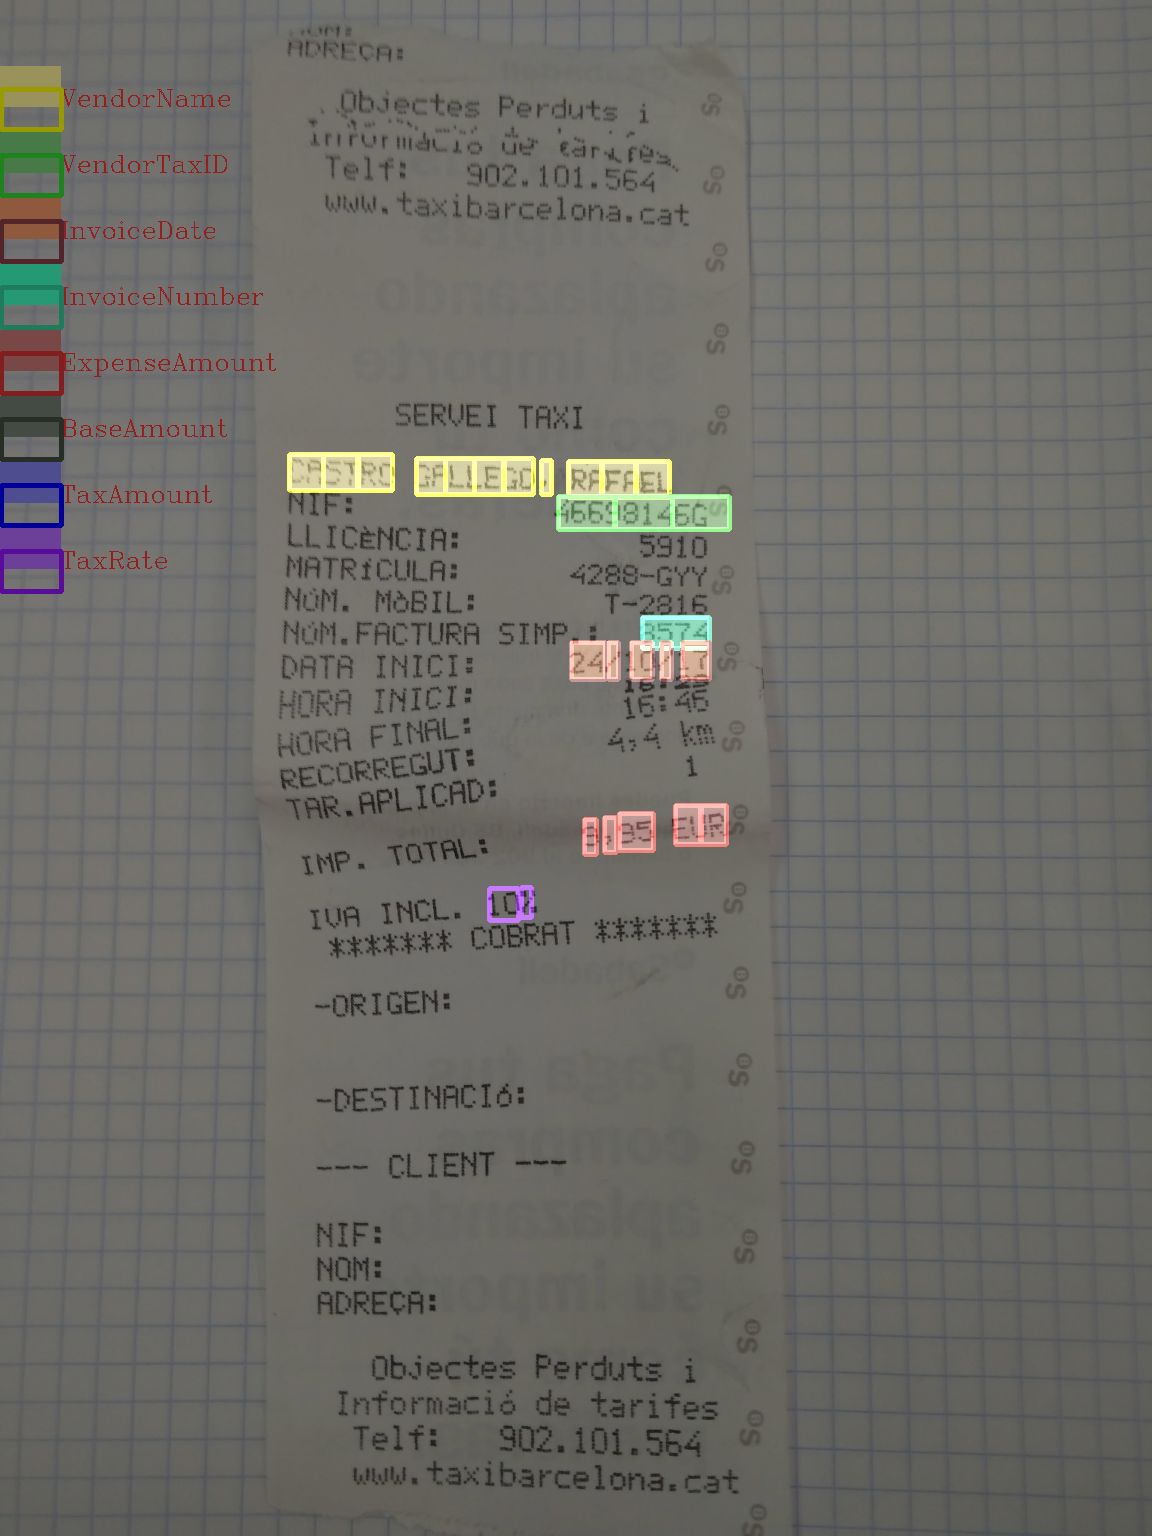
\includegraphics[width=0.31\linewidth]{appendix/taxi/FalseLabel_4.png}}\\
\subfloat{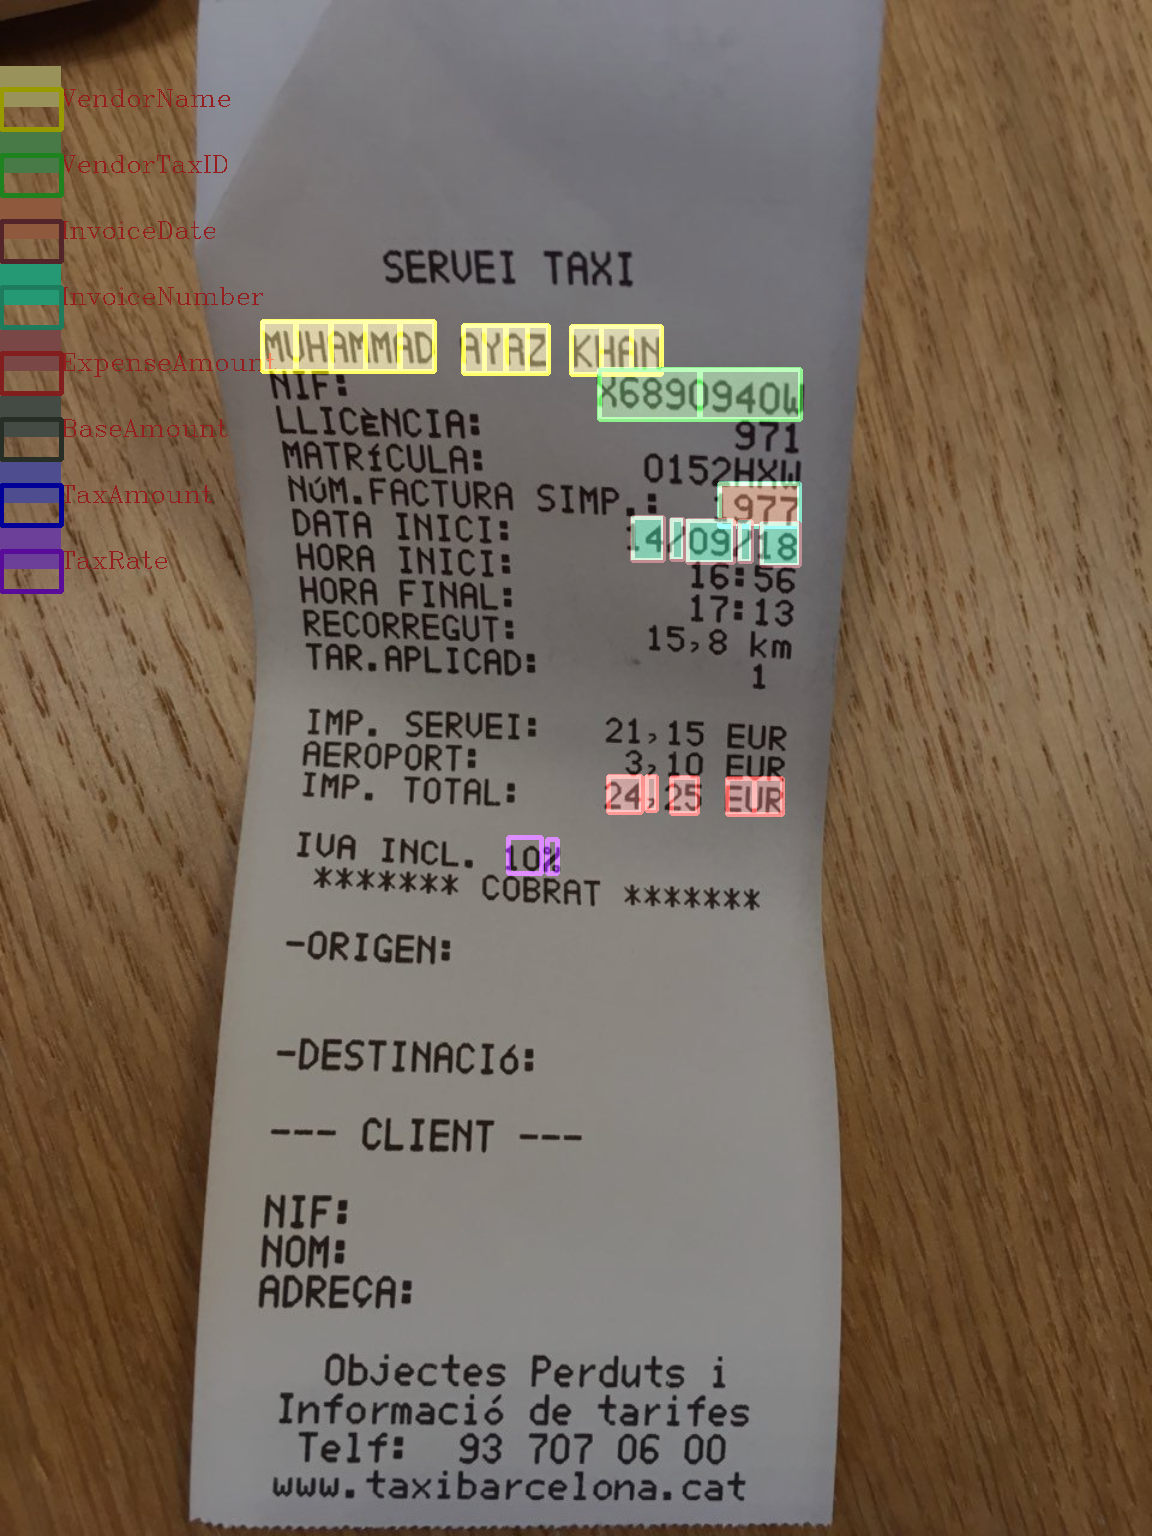
\includegraphics[width=0.36\linewidth]{appendix/taxi/FalseLabel_0.png}} 
\subfloat{\fcolorbox{white}{white}{}}
\subfloat{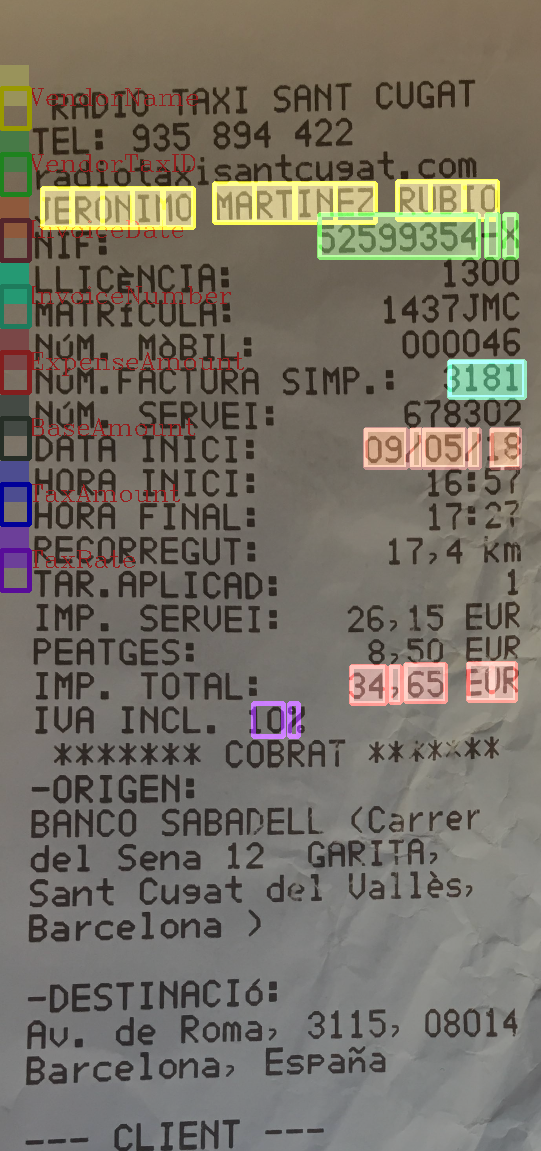
\includegraphics[width=0.22\linewidth]{appendix/taxi/FalseLabel_5.png}}
\subfloat{\fcolorbox{white}{white}{}}
\subfloat{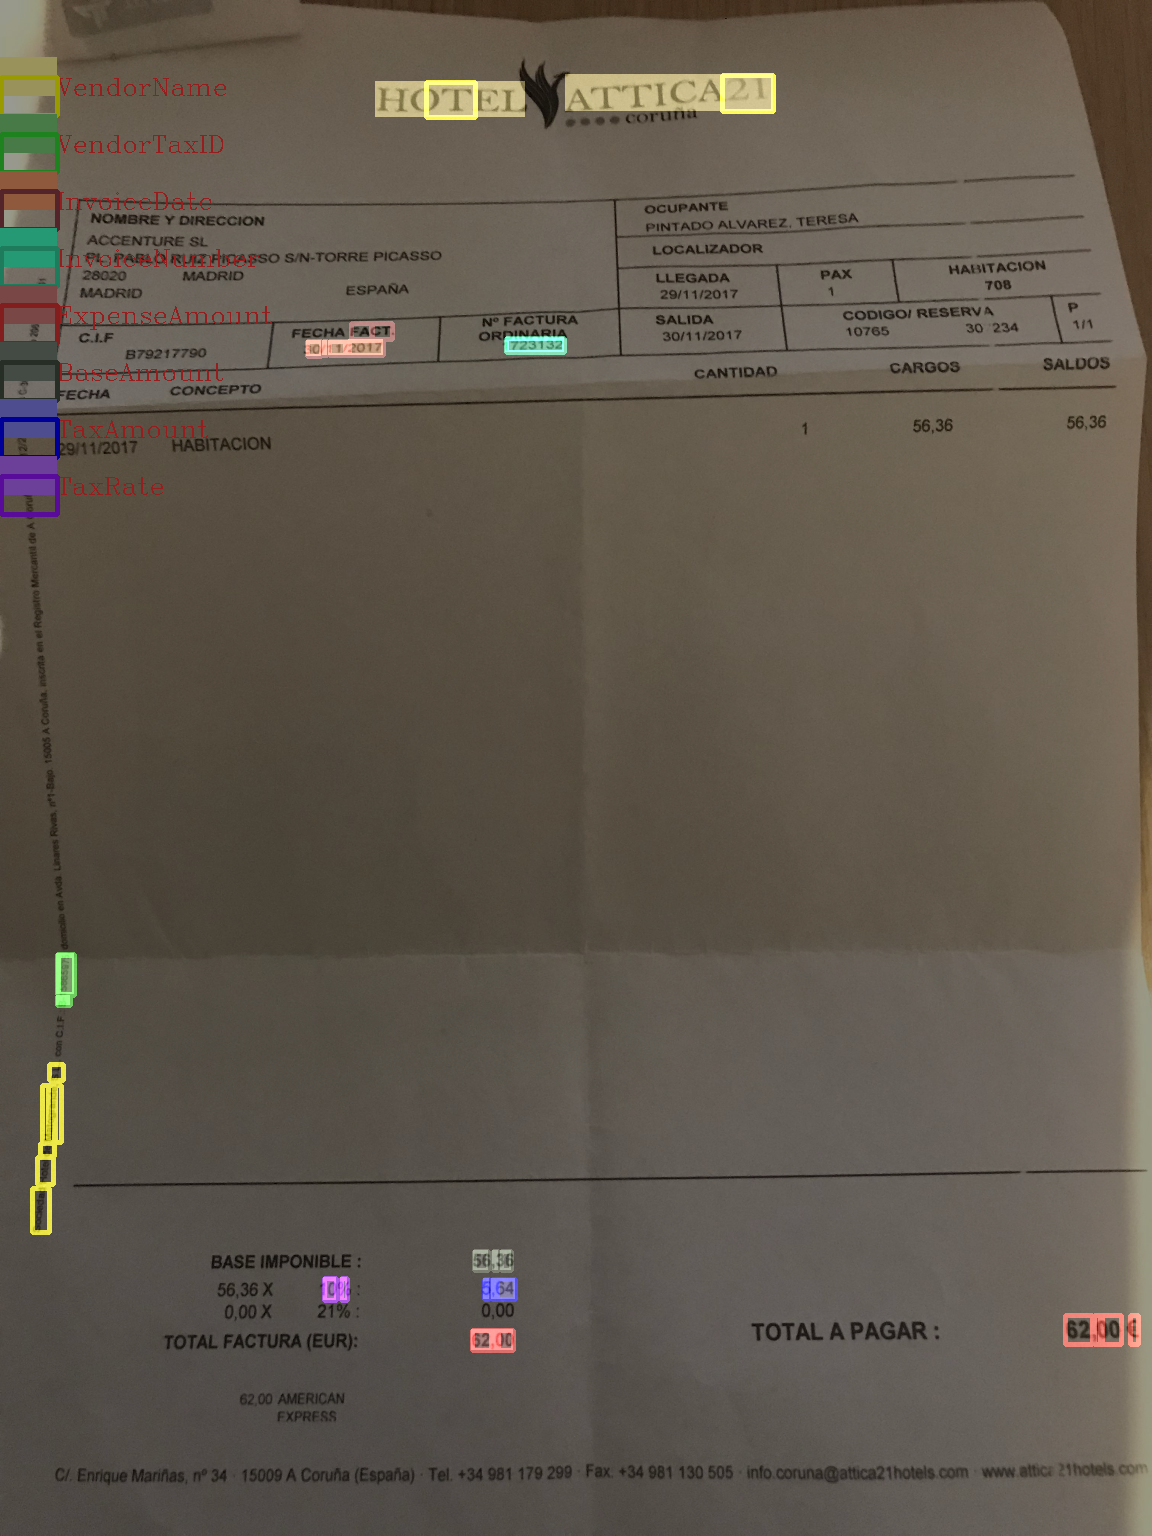
\includegraphics[width=0.36\linewidth]{appendix/hotel/FalseLabel_1.png}}\\
\end{center}
   \caption{False positive examples of CUITE prediction results, where the error is actually caused by the wrong labelling of human labeler. Color legend in the top-left corner indicates the key information classes. Each color indicates a key information class, where filled rectangles are the ground truths while the boundary-only rectangles are the inference results.}
\label{fig:falselabel}
\end{figure}


\subsection{Ablation Studies}
Although we have demonstrated extremely strong empirical results, the results presented are achieved by combination of each aspect of the CUTIE framework. In this section, we perform ablation studies over a number of facets of CUTIE in order to better understand their relative importance.

\subsubsection{Effect of Grid Augmentation on Understanding Spatial Information}
One of our core claim is that the high performance CUTIE is achieved by jointly analysis of the semantical and spatial information with the proposed framework. The highly effective spatial analysis ability is enabled by the CUTIE framework in contrast with the previous NER based methods. The grid augmentation process further enhances this ability. To give evidence to this claim, we evaluate CUTIE with or without the grid augmentation process. Results are presented in Table \ref{tab:augmentation}. We can see that adding grid augment process in CUTIE can significantly improve the performance on all of these receipts. These results demonstrate that CUTIE can greatly benefit from enhancing data diversity in spatial distribution. For that reason, further analysis about grid augmentation techniques will surely further enhance CUTIE's performance, \eg, randomly moving certain texts upward, downward, leftward, or rightward by several pixels during the grid positional mapping process. 
\begin{table}
	\caption{Performance evaluation of CUTIE with or without the grid augmentation process. (AP / softAP)}
\begin{center}
\begin{tabular}{l | c | c | c}
	 & Taxi & ME & Hotel \\
	\hline
	w augmentation & / & / & \\
	w/o augmentation & / & / & \\
\end{tabular}
\end{center}
	\label{tab:augmentation}
\end{table}

\subsubsection{Impact of Semantical Information Capacity}
Next, we evaluate the impact of semantical information of CUTIE by comparing evaluation with different word embedding sizes, although it is intuitively clear that larger embedding size provides more semantic capacity. As reported in Table \ref{tab:embedding}, CUTIE performs worse with smaller embedding size. The result meets our expectation that $details$. To further enhance the model performance, it might help to randomly mask out certain texts during the grid positional mapping process, such that the model learns inter-text relationship better with / without certain words present in the grid and further improves in generality.
\begin{table}
	\caption{Performance evaluation of CUTIE with different embedding size. (AP / softAP)}
\begin{center}
\begin{tabular}{l | c | c | c}
	 & Taxi & ME & Hotel \\
	\hline
	64 & / & / & \\
	128 & / & / & \\
	256 & / & / & \\
\end{tabular}
\end{center}
	\label{tab:embedding}
\end{table}

\subsubsection{Impact of Number of Training Samples}
To evaluate the impact of different number of training samples on model performance, we train CUTIE with $30\%$, $39\%$, $48\%$, $57\%$, $66\%$, and $75\%$ of our dataset, and report the results in Table \ref{tab:samples}.
\begin{table}
	\caption{Performance evaluation of CUTIE with different number of training samples. (AP / softAP)}
\begin{center}
\begin{tabular}{l | c | c | c}
	 & Taxi & ME & Hotel \\
	\hline
	30\% & / & / & \\
	39\% & / & / & \\
	48\% & / & / & \\
	57\% & / & / & \\
	66\% & / & / & \\
	75\% & 84.3 / 91.5 & \textbf{92.8} / \textbf{98.0} & 70.8 / \textbf{83.8} \\
\end{tabular}
\end{center}
	\label{tab:samples}
\end{table}

\section{Discussion}
Automatically extracting interested words / information from the scanned document images is of great interest to various services and applications. This paper proposes CUTIE to tackle this problem without requirement of any pre-training of post processing. Experimental results verifies the effectiveness of the proposed method. In contrast to the previous methods, the proposed method is easy to train and requires much smaller amount of training data while achieving state of the art performance. The performance gain is mainly achieved by exploring three key factors: the spatial relationship among texts, the semantic information of texts, and the grid positional mapping mechanism. One interesting finding is that the trained CUTIE model correctly predicts certain key information that is neglected to be labelled by the human labeler, which further proves the effectiveness of the proposed method. It is also worth mention that incorporating better semantical feature processing module or involving image-level features may further boost the model performance and we leave it to future research.

{\small
\bibliographystyle{ieee}
\bibliography{biblio}
}

\section{APPENDIX}
\subsection{Model Structure}
We report the best performed CUTIE-B model in Table \ref{tab:cutie}. Tokens are firstly embedd into $128$ dimensional features. Then, $4$ consecutive convolution operations are conducted in the conv block and $4$ consecutive atrous convolution are conducted in the atrous conv block with stride $1$ and rate $2$. Following the atrous conv block, an ASPP module is employed to combine multi-resolution features. The low level but high resolution feature from the $1$st output of the convolution block is also added to the model in the shortcut layer with a concatenation operation and a $1\times1$ convolution. Finally, inference result is achieved through a $1\times1$ convolution.
\begin{table}
	\caption{Structure of the proposed CUTIE-B model. }
\begin{center}
\begin{tabular}{l | c | c | c | c}
	layer name & operations & input dimension & output diemnsion & comments \\
	\hline
	embedding layer & - & 20000 & 128 & \\
	conv block & [$3\times5$]$\times$4 & 256 & 256 & stride=1 \\
	atrous conv block & [$3\times5$]$\times$4 & 256 & 256 & stride=1, rate=2 \\
	ASPP module & [$3\times5$]$\times$3, global pooling, concat, $1\times1$ & 256 & 256 & stride=1, rate=\{4,8,16\} \\
	shorcut layer & concat, $1\times1$ & 256 & 64 & \\
	output layer & $1\times1$ & 64 & 9 & \\ 
\end{tabular}
\end{center}
	\label{tab:cutie}
\end{table}

\end{document}
